\documentclass[10pt]{beamer}

\usetheme[progressbar=frametitle]{metropolis}
\usepackage{appendixnumberbeamer}

\usepackage{booktabs}
\usepackage[scale=2]{ccicons}

\usepackage{pgfplots}
\usepgfplotslibrary{dateplot}

\usepackage{xspace}
\newcommand{\themename}{\textbf{\textsc{metropolis}}\xspace}

% Packages added by Karl
\usepackage{wrapfig}
\input{USAmap.tex}
\usepackage{fancyvrb}
%\usepackage[dvipsnames]{xcolor}
\usepackage{colortbl}

\setlength{\arrayrulewidth}{.3mm}


\title{What Works?:}
\subtitle{Quasi-experiments in Cybersecurity Policy Interventions}
\date{\today}
\author{Karl Grindal, PhD Candidate}
\institute{Georgia Institute of Technology}
% \titlegraphic{\hfill\includegraphics[height=1.5cm]{logo.pdf}}

\begin{document}

\maketitle

\begin{frame}{Introduction}
  \setbeamertemplate{section in toc}[sections numbered]
  \tableofcontents%[hideallsubsections]
\end{frame}

\section{Introduction}

\begin{frame}{What is a breach notification letter?}
  \begin{figure}
	\includegraphics[width=\textwidth]{Figures/GT_Notification Letter_CA_highlight_all.jpg}
    \end{figure}
\end{frame}

\begin{frame}{Policy Literature}
Policy Evaluation
\begin{itemize}
    \item Romanosky et al. (2011) connected data breach notification laws to a 2\% reduction in identity theft. \cite{Romanoskydatabreachdisclosure2011a}
    \item Kesari (2020) noted that updates in 2016 to California data breach notification suggest ``.1 fewer reports per 100,000 people" for reported medical identity theft. \cite{KesariEffectStateData2020}
    \item  Liu (2020) found that state anti-phishing or credit freeze legislation did not impact annual identity theft reports. \cite{Liueffectstatecharacteristics2020}
\end{itemize}
The economics of information security is more fully developed, with the annual World Economics of Information Security (WEIS) conference serving as a focal point.

\end{frame}

\begin{frame}{Motivation}
\begin{quote}
One promising technique for the evaluation of some cybersecurity programs is the use of natural and quasi-natural experiments.
\end{quote}
\begin{quote}
Using a difference-in-differences methodology, one could conduct a quasi-natural experiment to determine the impact of mandatory data breach notification laws and regulations in the United States.
\end{quote}
\begin{flushright}
 -Benjamin Dean, 2016 \cite{BenjaminDeanNaturalQuasiNaturalExperiments}
\end{flushright}
\end{frame}

\begin{frame}{Research Question and Hypothesis}
\textbf{Research Question:} Have regulatory cyber policy interventions effectively reduced the frequency of data breach incidents \textit{ceteris paribus}? \\
\end{frame}

\begin{frame}{Research Question and Hypothesis}
\textbf{Research Question:} Have regulatory cyber policy interventions reduced the frequency of data breach incidents \textit{ceteris paribus}? \\
\begin{itemize}[<+- | alert@+>]
\item \textbf{Hypothesis 1:} The NY Department of Financial Services cybersecurity regulations reduced the frequency of reported data breaches in the New York financial sector.
\item \textbf{Hypothesis 2:} The Massachusetts Data Security Law reduced the frequency of reported data breaches in Massachusetts. \\
\item \textbf{Hypothesis 3:} The HITECH Act reduced the frequency of reported data breaches in the healthcare sector. \\
\item \textbf{Hypothesis 4:} The expansion of FTC Section 5 enforcement authority with the Wyndham Hotels suit reduced the frequency of reported data breaches nationally.

\end{itemize}
\end{frame}


\begin{frame}{Case Selection}
\begin{table}[h!]
    \begin{center}
    \label{tab:table1}
    \begin{tabular}{|p{2.5cm}|p{3.5cm}|p{3.5cm}|}
        \hline
        & \textbf{State Level} & \textbf{National Level} \\ \hline
      \textbf{Industry Wide Regulations} & NY DFS cybersecurity regulation (March 1, 2017) & HITECH Act, part of the ARRA (February 17, 2009) \\ \hline
      \textbf{Economy Wide Regulations} & Massachusetts Data Security Standard - 201 C.M.R. 17 (March 1, 2010) & FTC Section 5: Unfair or Deceptive Acts or Practices (Enforcement 2005-2020) \\
      \hline
    \end{tabular}
  \end{center}
\end{table}
\end{frame}


\section{Data Collection}


\begin{frame}{States with Breach Data Available}
    \begin{figure}
    \caption{States with Collected Data Breach Notification Information} \label{fig:map1}
    \resizebox{\textwidth}{!}{
    \begin{tikzpicture}{legend style={font=\small, at={(0.5,-.3)},anchor=north}}

    \tikzset{set state val/.style args={####1/####2}{####1={fill=orange!####2}}}
    \tikzset{set state val/.list={CA/90,CT/60,DE/90,FL/25,HI/90,ID/60,IA/90,IN/60,MA/60,MD/90,ME/60,MT/90,NC/60,ND/90,NE/60,NH/90,NJ/60,NM/25,NY/25,OR/60,RI/60,SC/60,VA/60,VT/90,WA/90,WI/60}}
    
    \USA[every state={draw=white, ultra thick, fill=black!10}]
    \matrix [draw,below left] at (current bounding box.north west) {
    \node [fill=orange!25,label=right:Notification Letters] {}; \\
    \node [fill=orange!60,label=right:Metadata] {}; \\
    \node [fill=orange!90,label=right:Both] {}; \\
    };
    \end{tikzpicture}
        }
    \end{figure}
\end{frame}

\begin{frame}{State Data - Percent of Collection for each Year}
\begin{table}[!h]
    \tabcolsep 3pt
    \label{tab:statedata}
    \resizebox{\textwidth}{!}{
\begin{tabular}{|l|c|c|c|c|c|c|c|c|c|c|c|c|c|c|c|c|}
  \hline
    \textbf{State} & \textbf{'05} & \textbf{'06} & \textbf{'07} & \textbf{'08} & \textbf{'09} & \textbf{'10} & \textbf{'11} & \textbf{'12} & \textbf{'13} & \textbf{'14} & \textbf{'15} & \textbf{'16} & \textbf{'17} & \textbf{'18} & \textbf{'19} & \textbf{'20}\\
  \hline  
  North Carolina & 85 & 100 & 100 & 100 & 100 & 100 & 100 & 100 & 100 & 100 & 100 & 100 & 100 & 90 & & \\
    \hline 
  New Hampshire &  & 53 & 100 & 100 & 100 & 100 & 100 & 100 & 100 & 100 & 100 & 100 & 100 & 100 & 100 & 83 \\
    \hline
  Hawaii & & & 47 & 100 & 100 & 100 & 100 & 100 & 100 & 100 & 100 & 100 & 100 & 100 & 100 & 30 \\
    \hline
  Massachusetts & & & 46 & 100 & 100 & 100 & 100 & 100 & 100 & 100 & 100 & 100 & 100 & 100 & 100 & 69  \\
    \hline
  South Carolina & & & & 43 & 100 & 100 & 100 & 100 & 100 & 100 & 100 & 100 & 100 & 100 & 48 & \\
    \hline
  Maine & & & & 42 & 100 & 100 & 100 & 100 & 100 & 100 & 100 & 100 & 100 & 100 & 100 & 70 \\
    \hline
  Iowa & & & & & & & 80 & 100 & 100 & 100 & 100 & 100 & 100 & 100 & 100 & 67 \\
    \hline
  California & & & & & & & & 95 & 100 & 100 & 100 & 100 & 100 & 100 & 100 & 70 \\
    \hline
  Wisconsin & & & & & & & & 69 & 100 & 100 & 100 & 100 & 100 & 100 & 100 & 54 \\
    \hline
  Connecticut & & & & & & & & 25 & 100 & 100 & 100 & 100 & 100 & 100 & 77 & \\
    \hline
  Virginia & & & & & & & & & 99 & 100 & 100 & 100 & 100 & 91 & & \\
    \hline
  Indiana &  & & & & & & & & 72 & 100 & 100 & 100 & 100 & 100 & 100 & 67 \\
    \hline
  Maryland &  & & & & & & & & & & 99 & 100 & 100 & 100 & 100 & 50 \\
    \hline
  Montana & & & & & & & & & & & 65 & 100 & 100 & 100 & 100 & 69 \\
    \hline
  Washington & & & & & & & & & & & 39 & 100 & 100 & 100 & 100 & 70 \\
    \hline
  Oregon &  & & & & & & & & &  & 17 & 100 & 100 & 100 & 100 & 71 \\
    \hline
  Rhode Island &  & & & & & & & & & & & 24 & 100 & 100 & 100 & 73 \\
    \hline
  Vermont &  & & & & & & & & & & & & 87 & 100 & 100 & 63 \\
    \hline   
  New Jersey &  & & & & & & & & & & & & 58 & 100 & 42 & \\
    \hline   
    Delaware &  & & & & & & & & & & & &  & 72 & 100 & 66 \\
    \hline   
  North Dakota &  & & & & & & & & & & & & & &  99 & 71 \\
    \hline
\end{tabular}}
\end{table}
\end{frame}


\begin{frame}{Descriptive Statistics for Collected }
\begin{table}[!h]
Descriptive Statistics of Captured Incidents
    \tabcolsep 2pt
    \label{tab:datasets1}
\begin{tabular}{|c|c|}
  \hline
  \textbf{Statistics} & \textbf{Measure}  \\
  \hline
  Number of captured incidents & 54,340 \\
  \hline
  Incidents dropped for No Reported Date & 559 \\
  Incidents dropped for Amended Submission & 45 \\
  Incidents dropped for Unclear Org Name & 14 \\
  \hline
  Incidents remaining after drops & 53,722 \\
  \hline
  Breaches after incident matching & 19,592 \\
  \hline
\end{tabular}
\end{table}

\end{frame}

\begin{frame}{Comparable Datasets}
\begin{table}[!h]
Datasets Used in Academic Research
    \tabcolsep 3pt
    \label{tab:datasets1}
    \resizebox{\textwidth}{!}{
\begin{tabular}{|p{1.8in}|c|c|c|c|c|}
  \hline
  \textbf{Dataset} & \textbf{Public} & \textbf{Collection Years} & \textbf{Comprehensive} & \textbf{Incidents} & \textbf{State} \\
  \hline
  \href{https://www.advisenltd.com/data/cyber-loss-data/}{Advisen Ltd} & N & '90-'19 & N & 150,000 \footnote{Hogan et al. (2020) \cite{HoganComprehensiveAnalysisCyber2020}} & N/A \\
  \hline
  \href{http://www.datalossdb.org}{Dataloss DB} & Y & '05-'15 & N & 1,078 & N \\
  \hline
  \href{http://www.hackmageddon.com}{Hackmageddon} & Y & '11-'20 & N & 613\footnote{Werner et al (2017) used 10 months in 2016 \cite{WernerTimeseriesforecasting2017}} & N \\
  \hline
  \href{https://www.hhs.gov/hipaa/for-individuals/medical-records/index.html}{HHS Breaches} & Y & '09-'20 & Y & 3,654\footnotemark[3] & Y \\
  \hline
  \href{http://www.privacyrights.org}{Privacy Rights Clearinghouse} & Y & '05-'19 & N & 9,015\footnotemark[3] & Y \\
  \hline
  SAS® OpRisk Global Data & N &  '95-'14 & N & 26,541 & N/A \\
  \hline
  \href{http://www.veriscommunity.net/index.html}{Veris Community} & Y & '98-'20 & N & 7,833\footnote{Updated December 12, 2020} & Y/N \\
  \hline
\end{tabular}}
\end{table}
\begin{table}[!h]
New Breach Data
    \tabcolsep 3pt
    \label{tab:dataset2}
    \resizebox{\textwidth}{!}{
\begin{tabular}{|p{1.8in}|c|c|c|c|c|}
  \hline
  \textbf{Dataset} & \textbf{Public} & \textbf{Collection Years} & \textbf{Comprehensive} & \textbf{Incidents} & \textbf{State} \\
  \hline
  My State Breach Data & Y & '05-'20 & Y & 19,592 & Y \\
  \hline
\end{tabular}}
\end{table}
\end{frame}

\section{Methodology}


\begin{frame}{Diagram of Factor Relationships}
    \begin{figure}
   \label{fig:diagram}
	\includegraphics[width=\textwidth]{Figures/Breach_FlowChart_v1.png}
	\caption{\small * includes Cyber Hygine, Government Capability, Vulnerabilities, etc.} 
    \end{figure}
\end{frame}

\begin{frame}{Regulatory Enforcement}
\begin{table}[!htb]
  \caption{First Regulatory Enforcement}
  \resizebox{\textwidth}{!}{
  \label{tab:comp_penalties}
\begin{tabular}{lccc}
\hline
State Law                                                        & \multicolumn{1}{l}{\begin{tabular}[c]{@{}l@{}}Massachusetts Data \\ Security Law\end{tabular}} & \multicolumn{1}{l}{HITECH Act}                                                                         & \multicolumn{1}{l}{\begin{tabular}[c]{@{}l@{}}NY DFS \\ cyber regulations\end{tabular}}       \\ \hline \hline
\begin{tabular}[c]{@{}l@{}}First \\ Enforcement\end{tabular} & Briar Group & \begin{tabular}[c]{@{}c@{}}Blue Cross Blue \\ Shield of Tennessee\end{tabular}                         & \begin{tabular}[c]{@{}c@{}}Residential \\ Mortgage Inc.\end{tabular} \\ \hline
Scope of Incident & \begin{tabular}[c]{@{}c@{}}Hack lasted \\ 8 months, took \\ credit card data.\end{tabular}                                & \begin{tabular}[c]{@{}c@{}}Theft of hard drives\\  over 1 million \\ individuals affected\end{tabular} & \begin{tabular}[c]{@{}c@{}}Phishing attack \\ accessed mailing \\ list (unreported)\end{tabular} \\ \hline
Penalty  & \$110,000 & \$1,500,000 & \$1,500,000  \\ \hline
\begin{tabular}[c]{@{}l@{}}Days Since Regulation
\\ Has Been Enforced\end{tabular} & 372 days & 1,017 days & 1,112 days \\ \hline
\end{tabular}}
\end{table}
\end{frame}


\begin{frame}{Quasi-Experimental Research}
    Experimental Research
    \begin{itemize}
        \item The “gold-standard” of research is randomized controlled trials
        \item Random assignment helps to achieve identical treatment and control groups
        \item Can be costly to implement and is sometimes unethical
    \end{itemize}
    Quasi-Experimental Research
    \begin{itemize}
        \item An empirical interventional study with non-random assignment
        \item Allows for observational data to be used
        \item Statistical methodologies like interrupted time series and propensity matching can address some of the challenges associated with using nonequivalent groups
    \end{itemize}
\end{frame}


\begin{frame}{Quasi-Experimental Research}
Interrupted Time Series (ITS)
    \begin{itemize}
        \item Analysis of time series data (i.e., an outcome measured over time)
        \item Comparison of the outcome before and after an intervention
        \item This method is particularly useful for assessing the impact of changes in policy
    \end{itemize}

\begin{table}
    \tabcolsep 3pt
    \label{tab:its1}
    \resizebox{\textwidth}{!}{
\begin{tabular}{|p{1.3in}|c|c|c|}
  \hline
  \textbf{Group} & \textbf{Pre-Test} & \textbf{Treatment} & \textbf{Post-Test} \\
  \hline
    Experimental Group & $ \textit{O}_1\hspace{.5mm}O_2\hspace{.5mm}O_3\hspace{.5mm}O_4\hspace{.5mm}O_5\hspace{.5mm}O_ 6 $ & X & $ \textit{O}_7\hspace{.5mm}O_8\hspace{.5mm}O_9\hspace{.5mm}O_{10}\hspace{.5mm}O_{11}\hspace{.5mm}O_{12} $ \\
  \hline
\end{tabular}}
\end{table}
\end{frame}

\begin{frame}{Quasi-Experimental Research}
Comparative Design ITS
    \begin{itemize}
        \item Improves on ITS by comparing with a control series (i.e., no intervention)
        \item Comparative Design ITS has additional pre- and post-treatment measurements
        \item These additional measurements allow for segmented regression and comparison of changes in both level and slope
    \end{itemize}

\begin{table}
    \tabcolsep 3pt
    \label{tab:its2}
    \resizebox{\textwidth}{!}{
\begin{tabular}{|p{1.3in}|c|c|c|}
  \hline
  \textbf{Group} & \textbf{Pre-Test} & \textbf{Treatment} & \textbf{Post-Test} \\
  \hline
    Experimental Group & $ \textit{O}_1\hspace{.5mm}O_2\hspace{.5mm}O_3\hspace{.5mm}O_4\hspace{.5mm}O_5\hspace{.5mm}O_ 6 $ & X & $ \textit{O}_7\hspace{.5mm}O_8\hspace{.5mm}O_9\hspace{.5mm}O_{10}\hspace{.5mm}O_{11}\hspace{.5mm}O_{12}$  \\
  \hline
    Control Group & $ \textit{O}_{13}\hspace{.5mm}O_{14}\hspace{.5mm}O_{15}\hspace{.5mm}O_{16}\hspace{.5mm}O_{17}
    \hspace{.5mm}O_ {18}\hspace{.5mm}$ & & $ \textit{O}_{19}\hspace{.5mm}O_{20}\hspace{.5mm}O_{21}\hspace{.5mm}O_{22}
    \hspace{.5mm}O_{23}\hspace{.5mm}O_{24} $ \\
  \hline
\end{tabular}}
\end{table}
\end{frame}



\section{Findings}

\subsection{Minor Findings}

\begin{frame}{Overview of Minor Findings}
    Minor Findings
    \begin{itemize}
        \item The majority of reported incidents were localized in their effect.
        \item The number of individuals affected by a breach has an exponential distribution.
        \item There is a similar number of breaches per capita in states with similar reporting requirements. 
        \item Across all states, there is a slow but persistent rate of growth in breach incidents at approximately 20\% per year.
        \item The consistent seasonal variation observed in data breach reporting increased in the Spring and decreased in the Fall.

    \end{itemize}
\end{frame}

\begin{frame}{Number of Incidents Reported Across Different States}
\begin{figure}[!htb]
    
    \caption{Number of Incidents Reported Across Different States} \label{fig:statedistrib}
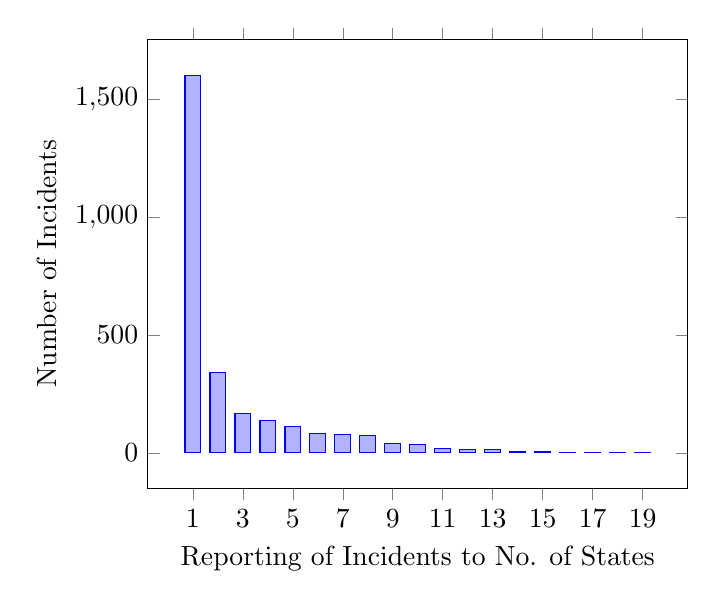
\begin{tikzpicture}  
\begin{axis}  
[  
    ybar,  
    bar width=0.2cm,
    enlarge y limits={abs=0.45cm},
    ylabel={Number of Incidents}, % the ylabel must precede a # symbol.  
    xlabel={Reporting of Incidents to No. of States},  
    symbolic x coords={1, 2, 3, 4, 5, 6, 7, 8, 9, 10, 11, 12, 13, 14, 15, 16, 17, 18, 19}, % these are the specification of coordinates on the x-axis.  
    xtick={1,3,5,7,9,11,13,15,17,19},
    nodes near coords align={vertical},  
    ]  
\addplot coordinates {(1,1603) (2,340) (3,169) (4,138) (5,112) (6,84) (7,79) (8,75) (9,41) (10,35) (11,20) (12,16) (13,13) (14,5) (15,5) (16,3) (17,1) (18,1) (19,2)};  
\end{axis}  
\end{tikzpicture}  
\end{figure}
\end{frame}

\begin{frame}{Total Individuals Affected By Breaches}
    \begin{figure}
    \caption{Histogram of Total Individuals Affected} \label{fig:hist_freq}
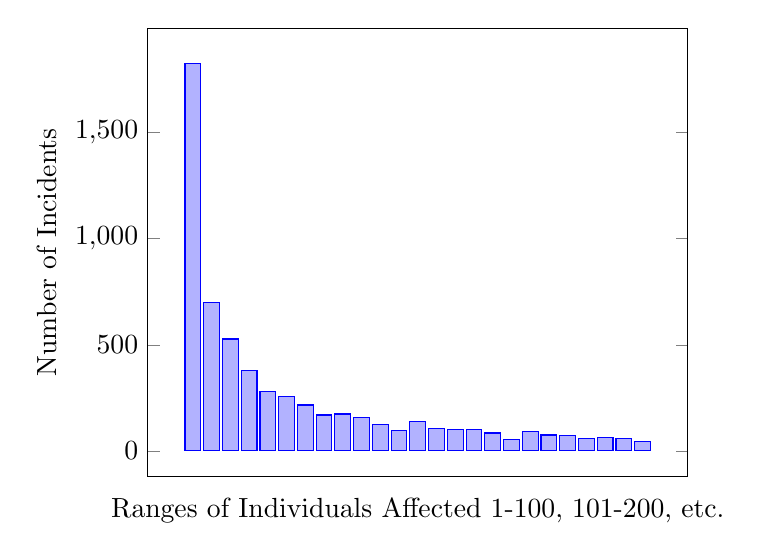
\begin{tikzpicture}  
\begin{axis}  
[   xtick=\empty,
    ybar,  
    bar width=0.2cm,
    enlarge y limits={abs=0.45cm},
    ylabel={Number of Incidents}, % the ylabel must precede a # symbol.  
    xlabel={Ranges of Individuals Affected 1-100, 101-200, etc.},  
    symbolic x coords={1, 2, 3, 4, 5, 6, 7, 8, 9, 10, 11, 12, 13, 14, 15, 16, 17, 18, 19, 20, 21, 22, 23, 24, 25}, % these are the specification of coordinates on the x-axis.  
    %xtick={1,5,9,13,17,21,25},
    nodes near coords align={vertical},  
    ]  
\addplot coordinates {(1,1825) (2,698) (3,527) (4,380) (5,281) (6,257) (7,216) (8,169) (9,174) (10,156) (11,123) (12,98) (13,140) (14,105) (15,99) (16,101) (17,84) (18,55) (19,90) (20,75) (21,73) (22,59) (23,63) (24,57) (25,46)};  
  
\end{axis}  
\end{tikzpicture}  

\end{figure}
\end{frame}

\begin{frame}{Breaches per Million}
    \begin{figure}
      \caption{Reported Breaches each Year per Million with No Resident Limits} \label{fig:figure15}
    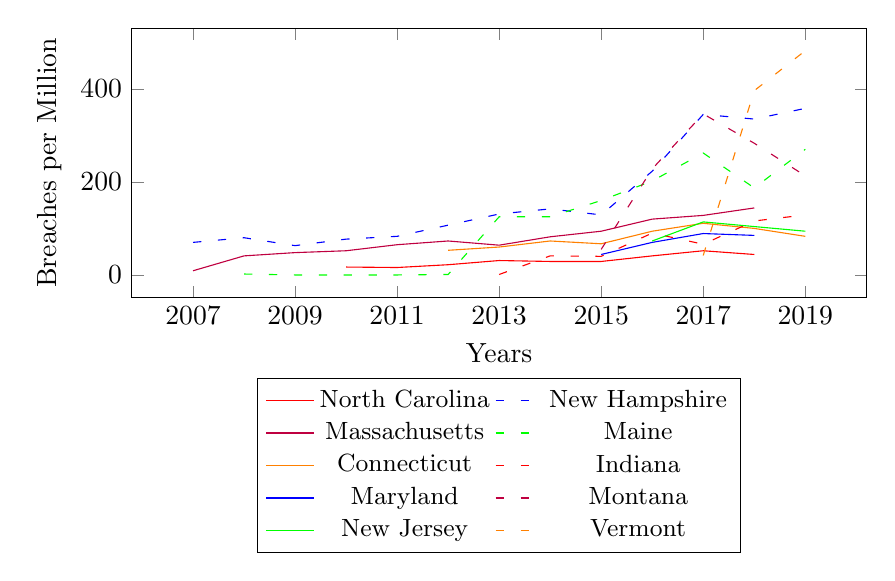
\begin{tikzpicture}
    \begin{axis}[legend columns=2, legend style={font=\small, at={(0.5,-.3)},anchor=north},
    xlabel={Years},
    ylabel={Breaches per Million},
    width=0.9\textwidth,
    height=5cm,
    symbolic x coords={2007,2008,2009,2010,2011,2012,2013,2014,2015,2016,2017,2018,2019}
    ]
    \addplot[color=red,]
    coordinates{(2007,) (2008,) (2009,) (2010,17) (2011,16) (2012,22) (2013,31) (2014,29) (2015,29) (2016,41) (2017,52) (2018,44) (2019,)};
    \addplot[color=blue,loosely dashed]
    coordinates{(2007,70) (2008,80) (2009,63) (2010,77) (2011,83) (2012,107) (2013,131) (2014,142) (2015,129) (2016,223) (2017,345) (2018,335) (2019,358)};
    \addplot[color=purple,]
    coordinates{(2007,9) (2008,41) (2009,48) (2010,52) (2011,65) (2012,73) (2013,64) (2014,82) (2015,94) (2016,120) (2017,128) (2018,144) (2019,)};
    \addplot[color=green,loosely dashed]
    coordinates{(2007,) (2008,2) (2009,0) (2010,0) (2011,0) (2012,1) (2013,125) (2014,125) (2015,160) (2016,202) (2017,262) (2018,187) (2019,270)};
    \addplot[color=orange,]
    coordinates{(2007,) (2008,) (2009,) (2010,) (2011,) (2012,53) (2013,60) (2014,73) (2015,67) (2016,94) (2017,111) (2018,100) (2019,83)};
    \addplot[color=red,loosely dashed]
    coordinates{(2007,) (2008,) (2009,) (2010,) (2011,) (2012,) (2013,1) (2014,41) (2015,40) (2016,90) (2017,66) (2018,116) (2019,129)};
    \addplot[color=blue,]
    coordinates{(2007,) (2008,) (2009,) (2010,) (2011,) (2012,) (2013,) (2014,) (2015,44) (2016,70) (2017,89) (2018,85) (2019,)};
    \addplot[color=purple,loosely dashed]
    coordinates{(2007,) (2008,) (2009,) (2010,) (2011,) (2012,) (2013,) (2014,) (2015,55) (2016,228) (2017,346) (2018,283) (2019,213)};
    \addplot[color=green,]
    coordinates{(2007,) (2008,) (2009,) (2010,) (2011,) (2012,) (2013,) (2014,) (2015,) (2016,73) (2017,114) (2018,104) (2019,94)};
    \addplot[color=orange,loosely dashed]
    coordinates{(2007,) (2008,) (2009,) (2010,) (2011,) (2012,) (2013,) (2014,) (2015,) (2016,) (2017,42) (2018,396) (2019,482)};
    \legend{North Carolina, New Hampshire, Massachusetts, Maine, Connecticut, Indiana, Maryland, Montana, New Jersey, Vermont}
    \end{axis}
    \end{tikzpicture}
    \end{figure}
\end{frame}

\begin{frame}{Breaches per Million}
    \begin{figure}
      \caption{Reported Breaches each Year per Million with Resident Limits} \label{fig:figure16}
    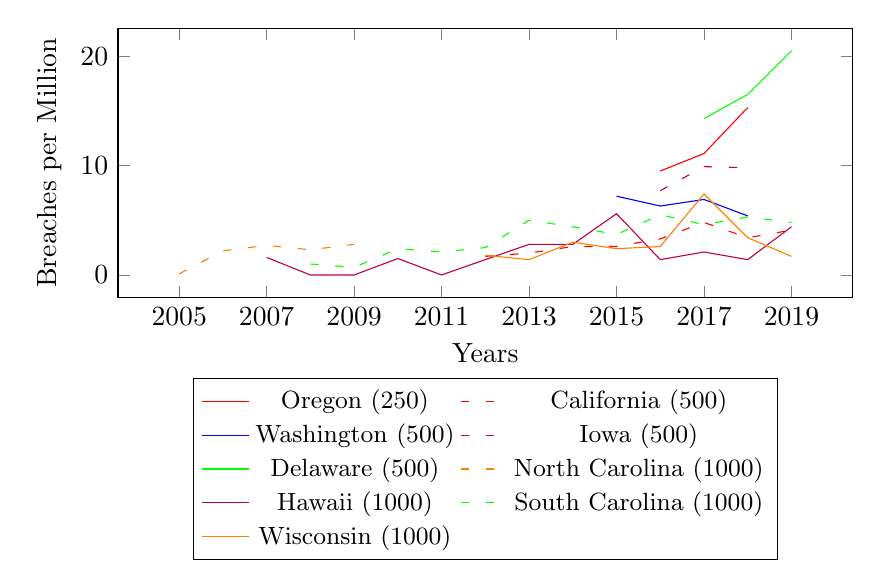
\begin{tikzpicture}
    \begin{axis}[legend columns=2, legend style={font=\small, at={(0.5,-.3)},anchor=north},
    xlabel={Years},
    ylabel={Breaches per Million},
    width=0.9\textwidth,
    height=5cm,
    symbolic x coords={2005,2006,2007,2008,2009,2010,2011,2012,2013,2014,2015,2016,2017,2018,2019}
    ]
    \addplot[color=red,] 
    coordinates{(2005,) (2006,) (2007,) (2008,) (2009,) (2010,) (2011,) (2012,) (2013,) (2014,) (2015,) (2016,9.5) (2017,11.1) (2018,15.3) (2019,)};
    \addplot[color=red,loosely dashed]
    coordinates{(2005,) (2006,) (2007,) (2008,) (2009,) (2010,) (2011,) (2012,1.7) (2013,2.0) (2014,2.6) (2015,2.6) (2016,3.3) (2017,4.8) (2018,3.4) (2019,4.1)};
    \addplot[color=blue,]
    coordinates{(2005,) (2006,) (2007,) (2008,) (2009,) (2010,) (2011,) (2012,) (2013,) (2014,) (2015,7.2) (2016,6.3) (2017,6.9) (2018,5.4) (2019,)};
    \addplot[color=purple,loosely dashed]
    coordinates{(2005,) (2006,) (2007,) (2008,) (2009,) (2010,) (2011,) (2012,) (2013,) (2014,) (2015,) (2016,7.7) (2017,9.9) (2018,9.8) (2019,)};
    \addplot[color=green,]
    coordinates{(2005,) (2006,) (2007,) (2008,) (2009,) (2010,) (2011,) (2012,) (2013,) (2014,) (2015,) (2016,) (2017,14.3) (2018,16.5) (2019,20.5)};
    \addplot[color=orange,loosely dashed]
    coordinates{(2005,.1) (2006,2.2) (2007,2.7) (2008,2.3) (2009,2.8) (2010,) (2011,) (2012,) (2013,) (2014,) (2015,) (2016,) (2017,) (2018,) (2019,)};
    \addplot[color=purple,]
    coordinates{(2005,) (2006,) (2007,1.6) (2008,0) (2009,0) (2010,1.5) (2011,0) (2012,1.4) (2013,2.8) (2014,2.8) (2015,5.6) (2016,1.4) (2017,2.1) (2018,1.4) (2019,4.4)};
    \addplot[color=green,loosely dashed]
    coordinates{(2005,) (2006,) (2007,) (2008,1.0) (2009,.7) (2010,2.4) (2011,2.1) (2012,2.5) (2013,5.0) (2014,4.4) (2015,3.7) (2016,5.5) (2017,4.6) (2018,5.3) (2019,4.8)};
    \addplot[color=orange,]
    coordinates{(2005,) (2006,) (2007,) (2008,) (2009,) (2010,) (2011,) (2012,1.8) (2013,1.4) (2014,3.0) (2015,2.4) (2016,2.6) (2017,7.4) (2018,3.4) (2019,1.7)};
    \legend{Oregon (250), California (500), Washington (500), Iowa (500), Delaware (500), North Carolina (1000),Hawaii (1000), South Carolina (1000), Wisconsin (1000)}
    \end{axis}
    \end{tikzpicture}
    \end{figure}
\end{frame}

\begin{frame}{Evidence for Seasonal Trends}
    \begin{figure}[!htb]
    \caption{Seasonal Variation in Breaches per Million} \label{fig:seasonalvar}
    {
    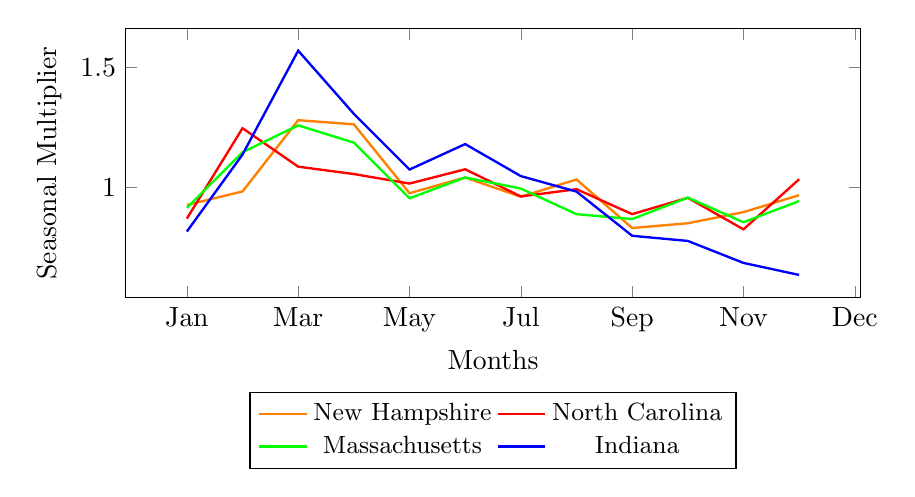
\begin{tikzpicture}
    \begin{axis}[legend columns=2, legend style={font=\small}, legend style={font=\small, at={(0.5,-.35)},anchor=north},
    xlabel={Months},
    ylabel={Seasonal Multiplier},
    width=0.9\textwidth,
    height=5cm,
    symbolic x coords={Jan,Feb,Mar,Apr,May,Jun,Jul,Aug,Sep,Oct,Nov,Dec}
    ]
    \addplot[line width=0.3mm, color=orange]
    coordinates{(Jan,0.9260406) (Feb,0.9823979) (Mar,1.2790158) (Apr,1.2617402) (May,0.9749716) (Jun,1.0403656) (Jul,0.9601914) (Aug,1.0321638) (Sep,0.8301902) (Oct,0.8498937) (Nov,0.8962966) (Dec,0.9667326)};
    
    \addplot[line width=0.3mm, color=red]
    coordinates{(Jan,0.8694024) (Feb,1.2455973) (Mar,1.0854986) (Apr,1.0548478) (May,1.0151817) (Jun,1.0746119) (Jul,0.9615493) (Aug,0.9916769) (Sep,0.8878670) (Oct,0.9559964) (Nov,0.8246104) (Dec,1.0331603)};

    \addplot[line width=0.3mm, color=green]
    coordinates{(Jan,0.9142141) (Feb,1.1456061) (Mar,1.2574376) (Apr,1.1854509) (May,0.9539506) (Jun,1.0405965) (Jul,0.9944509) (Aug,0.8877185) (Sep,0.8672905) (Oct,0.9566873) (Nov,0.8541875) (Dec,0.9424095)};

    \addplot[line width=0.3mm, color=blue]
    coordinates{(Jan,0.8153707) (Feb,1.1359828) (Mar,1.5684250) (Apr,1.3054371) (May,1.0735237) (Jun,1.1795521) (Jul,1.0462436) (Aug,0.9817047) (Sep,0.7978249) (Oct,0.7763317) (Nov,0.6848185) (Dec,0.6347853)};

    \legend{New Hampshire, North Carolina, Massachusetts, Indiana}
    \end{axis}
    \end{tikzpicture}}
\end{figure}
\end{frame}

\subsection{Major Findings}

\begin{frame}{Overview of Major Findings}    
    Major Findings
    \begin{itemize}
        \item The New York Department of Financial Services regulations was shown to be effective. The intervention lead to a reduction in 27 financial sector breaches in New York over the course of a year.
        \item In contrast, the Massachusetts Data Security Law, the HITECH Act, and FTC's Wyndham's Actions did not demonstrate a reduction in reported data breaches.
    \end{itemize}
\end{frame}


\begin{frame}{Comparing New York Finance to Not-New York Finance with Maine Data}
\begin{figure}[!htb]
      \caption{Comparing New York Finance to Not-New York Finance with Maine Data} \label{fig:nyfin_notny}
    {
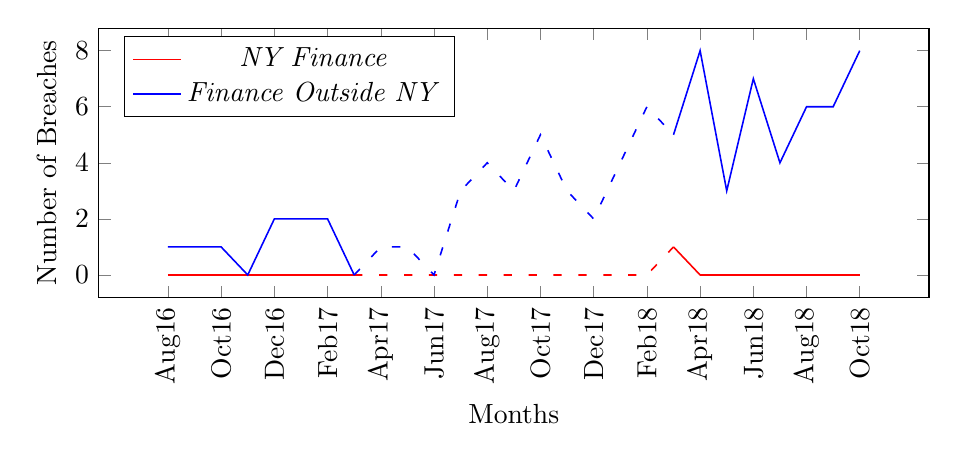
\begin{tikzpicture}
\begin{axis}[
  legend entries = {\textit{NY Finance},,,,,\textit{Finance Outside NY}}, legend pos=north west,
    xlabel={Months},
    ylabel={Number of Breaches},
    width=\textwidth,
    height=5cm,
    symbolic x coords={Aug16,Sep16,Oct16,Nov16,Dec16,Jan17,Feb17,Mar17,Apr17,May17,Jun17,Jul17,Aug17,Sep17,Oct17,Nov17,Dec17,Jan18,Feb18,Mar18,Apr18,May18,Jun18,Jul18,Aug18,Sep18,Oct18},
    xtick={Aug16,Oct16,Dec16,Feb17,Apr17,Jun17,Aug17,Oct17,Dec17,Feb18,Apr18,Jun18,Aug18,Oct18},
    x tick label style={rotate=90}
    ].
\addplot[line width=0.20mm,color=red]
    coordinates{(Aug16,0) (Sep16,0) (Oct16,0) (Nov16,0) (Dec16,0) (Jan17,0) (Feb17,0) (Mar17,0)
    };
\addplot[line width=0.20mm,color=red,loosely dashed]
    coordinates{(Mar17,0) (Apr17,0) (May17,0) (Jun17,0) (Jul17,0) (Aug17,0) (Sep17,0) (Oct17,0) (Nov17,0) (Dec17,0) (Jan18,0) (Feb18,0) (Mar18,1)
    };
\addplot[line width=0.20mm,color=red]
    coordinates{(Mar18,1) (Apr18,0) (May18,0) (Jun18,0) (Jul18,0) (Aug18,0) (Sep18,0) (Oct18,0)
    };
\addplot[line width=0.20mm,color=blue]
    coordinates{(Aug16,1) (Sep16,1) (Oct16,1) (Nov16,0) (Dec16,2) (Jan17,2) (Feb17,2) (Mar17,0)
    };
\addplot[line width=0.20mm,color=blue,loosely dashed]
    coordinates{(Mar17,0) (Apr17,1) (May17,1) (Jun17,0) (Jul17,3) (Aug17,4) (Sep17,3) (Oct17,5) (Nov17,3) (Dec17,2) (Jan18,4) (Feb18,6) (Mar18,5)
    };
\addplot[line width=0.20mm,color=blue]
    coordinates{(Mar18,5) (Apr18,8) (May18,3) (Jun18,7) (Jul18,4) (Aug18,6) (Sep18,6) (Oct18,8)
    };
\end{axis}
\end{tikzpicture}}
\end{figure}
\end{frame}


\begin{frame}{Comparative ITS NY DFS Regulations (NY Finance Compared to Non-NY Finance with Maine Data)}
    \begin{table}[!htb]
    \label{tab:MA_NYFin_NotNYFin}
    \resizebox{\textwidth}{!}{
    \begin{tabular}{l|c|c|r|l}
      \textbf{Parameter} & \textbf{Interpretation} & \textbf{Estimate} & \textbf{Std Error} & \textbf{Probability}\\ % <-- added & and content for each column
      \hline
      $\alpha$ & Intercept & 1.11 & 0.81 & 0.18 \\  \hline % <--
      $\beta_1$ & Control Pre-Trend & -0.02 & 0.16 & 0.88 \\  \hline % <--
      $\beta_2$ & Control Post-Level & 4.05 & 1.05 & 0.00 *** \\ % <--
      & Change & & & \\ \hline
      $\beta_3$ & Control Post-Trend & 0.23 & 0.23 & 0.34 \\ % <--
      & Change & & & \\ \hline
      $\beta_4$ & Treatment/Control & -1.11 & 1.14 & 0.34 \\ % <--
      & Pre-Level Difference & & & \\ \hline
      $\beta_5$ & Treatment/Control & 0.02 & 0.23 & 0.92 \\ % <--
            & Pre-Trend Difference & & & \\ \hline
\rowcolor{yellow}      $\beta_6$ & Treatment/Control & -3.55 & 1.48 & 0.02 * \\ % <--\
\rowcolor{yellow}            & Post-Level Difference & & & \\ \hline
\rowcolor{lightgray}      $\beta_7$ & Treatment/Control Change  & -0.31 & 0.31 & 0.34 \\ % <--
\rowcolor{lightgray}            & in Slope Difference Pre-to Post- & & & \\ \hline
    \end{tabular}}
\end{table}
\end{frame}


\begin{frame}{Comparing New York Finance to Not-New York Finance with Connecticut Data}
    \begin{figure}[!htb]
      \caption{Comparing New York Finance to Not-New York Finance with Connecticut Data} \label{fig:NYDFS_NotNY_CT}
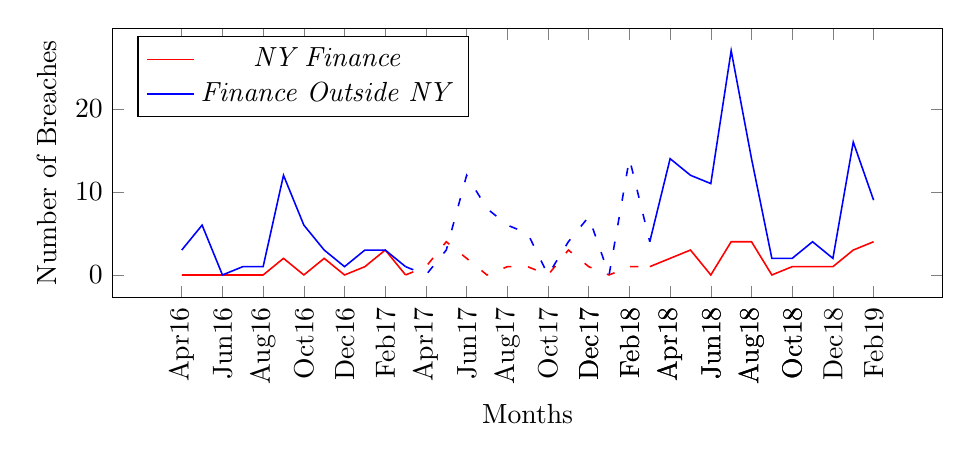
\begin{tikzpicture}
\begin{axis}[
  legend entries = {\textit{NY Finance},,,,,\textit{Finance Outside NY}}, legend pos=north west,
    xlabel={Months},
    ylabel={Number of Breaches},
    width=\textwidth,
    height=5cm,
    symbolic x coords={Apr16,May16,Jun16,Jul16,Aug16,Sep16,Oct16,Nov16,Dec16,Jan17,Feb17,Mar17,Apr17,May17,Jun17,Jul17,Aug17,Sep17,Oct17,Nov17,Dec17,Jan18,Feb18,Mar18,Apr18,May18,Jun18,Jul18,Aug18,Sep18,Oct18,Nov18,Dec18,Jan19,Feb19},
    xtick={Apr16,Jun16,Aug16,Oct16,Dec16,Feb17,Apr17,Jun17,Aug17,Oct17,Dec17,Feb18,Apr18,Jun18,Aug18,Oct18,Dec17,Feb18,Apr18,Jun18,Aug18,Oct18,Dec18,Feb19},
    x tick label style={rotate=90}
    ].
\addplot[line width=0.20mm,color=red]
    coordinates{(Apr16,0) (May16,0) (Jun16,0) (Jul16,0) (Aug16,0) (Sep16,2) (Oct16,0) (Nov16,2) (Dec16,0) (Jan17,1) (Feb17,3) (Mar17,0) 
    };
\addplot[line width=0.20mm,color=red,loosely dashed]
    coordinates{(Mar17,0) (Apr17,1) (May17,4) (Jun17,2) (Jul17,0) (Aug17,1) (Sep17,1) (Oct17,0) (Nov17,3) (Dec17,1) (Jan18,0) (Feb18,1) (Mar18,1)
    };
\addplot[line width=0.20mm,color=red]
    coordinates{(Mar18,1) (Apr18,2) (May18,3) (Jun18,0) (Jul18,4) (Aug18,4) (Sep18,0) (Oct18,1) (Nov18,1) (Dec18,1) (Jan19,3) (Feb19,4)
    };
\addplot[line width=0.20mm,color=blue]
    coordinates{(Apr16,3) (May16,6) (Jun16,0) (Jul16,1) (Aug16,1) (Sep16,12) (Oct16,6) (Nov16,3) (Dec16,1) (Jan17,3) (Feb17,3) (Mar17,1)
    };
\addplot[line width=0.20mm,color=blue,loosely dashed]
    coordinates{(Mar17,1) (Apr17,0) (May17,3) (Jun17,12) (Jul17,8) (Aug17,6) (Sep17,5) (Oct17,0) (Nov17,4) (Dec17,7) (Jan18,0) (Feb18,14) (Mar18,4) 
    };
\addplot[line width=0.20mm,color=blue]
    coordinates{(Mar18,4) (Apr18,14) (May18,12) (Jun18,11) (Jul18,27) (Aug18,14) (Sep18,2) (Oct18,2) (Nov18,4) (Dec18,2) (Jan19,16) (Feb19,9)
    };
    
\end{axis}
\end{tikzpicture}
\end{figure}
\end{frame}

\begin{frame}{Comparative ITS NY DFS Regulations (NY Finance Compared to NY Not-Finance with Connecticut Data)}
    \begin{table}[!htb]
    \label{tab:reg_NY_NotNYFin_CT}
    \resizebox{\textwidth}{!}{
    \begin{tabular}{l|c|c|r|l}
      \textbf{Parameter} & \textbf{Interpretation} & \textbf{Estimate} & \textbf{Std Error} & \textbf{Probability}\\ % <-- added & and content for each column
      \hline
      $\alpha$ & Intercept & 3.97 & 2.68 & 0.15 \\  \hline % <--
      $\beta_1$ & Control Pre-Trend & -0.10 & 0.36 & 0.79 \\  \hline % <--
      $\beta_2$ & Control Post-Level &  9.66 & 3.57 & 0.01 * \\ % <--
      & Change & & & \\ \hline
      $\beta_3$ & Control Post-Trend & -0.32 & 0.51 & 0.54 \\ % <--
      & Change & & & \\ \hline
      $\beta_4$ & Treatment/Control & -4.17 & 3.79 & 0.28 \\ % <--
      & Pre-Level Difference & & & \\ \hline
      $\beta_5$ & Treatment/Control & 0.23 & 0.51 & 0.66 \\ % <--
            & Pre-Trend Difference & & & \\ \hline
\rowcolor{yellow}      $\beta_6$ & Treatment/Control & -9.51 & 5.05 & 0.07 . \\ % <--\
\rowcolor{yellow}            & Post-Level Difference & & & \\ \hline
\rowcolor{lightgray}      $\beta_7$ & Treatment/Control Change  & 0.26 & 0.73 & 0.73 \\ % <--
\rowcolor{lightgray}            & in Slope Difference Pre-to Post- & & & \\ \hline
    \end{tabular}}
    \end{table}
\end{frame}


\begin{frame}{Comparing New York Finance to Not-New York Finance with Connecticut Data (First Date of Breach)}
    \begin{figure}[!htb]
    \caption{Comparing New York Finance to Not-New York Finance with Connecticut Data (First Date of Breach)}
      \label{fig:NYDFS_NotNY_CTRobust}
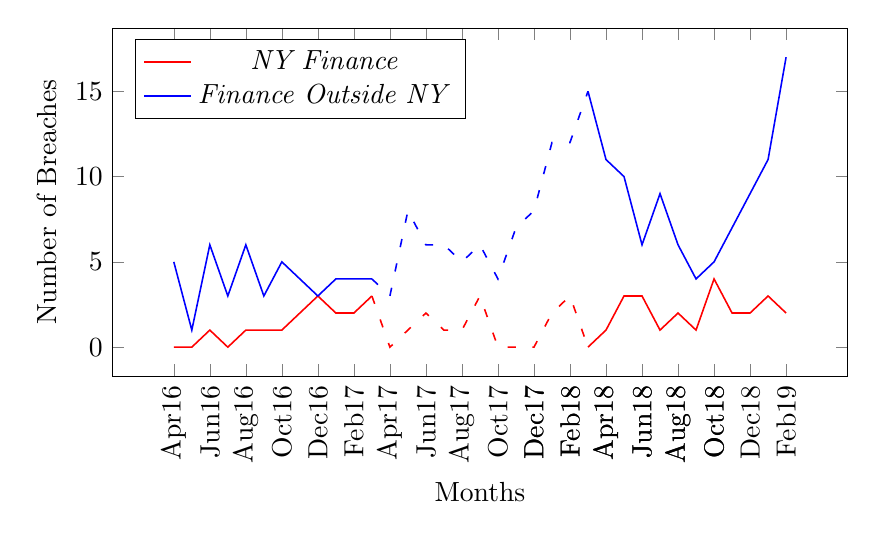
\begin{tikzpicture}
\begin{axis}[
  legend entries = {\textit{NY Finance},,,,,\textit{Finance Outside NY}}, legend pos=north west,
    xlabel={Months},
    ylabel={Number of Breaches},
    width=0.9\textwidth,
    height=6cm,
    symbolic x coords={Apr16,May16,Jun16,Jul16,Aug16,Sep16,Oct16,Nov16,Dec16,Jan17,Feb17,Mar17,Apr17,May17,Jun17,Jul17,Aug17,Sep17,Oct17,Nov17,Dec17,Jan18,Feb18,Mar18,Apr18,May18,Jun18,Jul18,Aug18,Sep18,Oct18,Nov18,Dec18,Jan19,Feb19},
    xtick={Apr16,Jun16,Aug16,Oct16,Dec16,Feb17,Apr17,Jun17,Aug17,Oct17,Dec17,Feb18,Apr18,Jun18,Aug18,Oct18,Dec17,Feb18,Apr18,Jun18,Aug18,Oct18,Dec18,Feb19},
    x tick label style={rotate=90}
    ].
\addplot[line width=0.20mm,color=red]
    coordinates{(Apr16,0) (May16,0) (Jun16,1) (Jul16,0) (Aug16,1) (Sep16,1) (Oct16,1) (Nov16,2) (Dec16,3) (Jan17,2) (Feb17,2) (Mar17,3) 
    };
\addplot[line width=0.20mm,color=red,loosely dashed]
    coordinates{(Mar17,3) (Apr17,0) (May17,1) (Jun17,2) (Jul17,1) (Aug17,1) (Sep17,3) (Oct17,0) (Nov17,0) (Dec17,0) (Jan18,2) (Feb18,3) (Mar18,0)
    };
\addplot[line width=0.20mm,color=red]
    coordinates{(Mar18,0) (Apr18,1) (May18,3) (Jun18,3) (Jul18,1) (Aug18,2) (Sep18,1) (Oct18,4) (Nov18,2) (Dec18,2) (Jan19,3) (Feb19,2)
    };
\addplot[line width=0.20mm,color=blue]
    coordinates{(Apr16,5) (May16,1) (Jun16,6) (Jul16,3) (Aug16,6) (Sep16,3) (Oct16,5) (Nov16,4) (Dec16,3) (Jan17,4) (Feb17,4) (Mar17,4)
    };
\addplot[line width=0.20mm,color=blue,loosely dashed]
    coordinates{(Mar17,4) (Apr17,3) (May17,8) (Jun17,6) (Jul17,6) (Aug17,5) (Sep17,6) (Oct17,4) (Nov17,7) (Dec17,8) (Jan18,12) (Feb18,12) (Mar18,15) 
    };
\addplot[line width=0.20mm,color=blue]
    coordinates{(Mar18,15) (Apr18,11) (May18,10) (Jun18,6) (Jul18,9) (Aug18,6) (Sep18,4) (Oct18,5) (Nov18,7) (Dec18,9) (Jan19,11) (Feb19,17)
    };
    
\end{axis}
\end{tikzpicture}
\end{figure}
\end{frame}


\begin{frame}{Comparative ITS NY DFS Regulations (NY Finance Compared to NY Not-Finance, Connecticut Robustness Check)}
\begin{table}[!htb]
    %\caption{Comparative ITS NY DFS Regulations (NY Finance Compared to NY Not-Finance, Connecticut Robustness Check)}
    \label{tab:reg_NY_NotNYFin_CT_First}
    \resizebox{\textwidth}{!}{
    \begin{tabular}{l|c|c|r|l}
      \textbf{Parameter} & \textbf{Interpretation} & \textbf{Estimate} & \textbf{Std Error} & \textbf{Probability}\\ % <-- added & and content for each column
      \hline
      $\alpha$ & Intercept & 4.05 & 1.40 & 0.01 ** \\  \hline % <--
      $\beta_1$ & Control Pre-Trend & -0.00 & 0.19 & 0.97 \\  \hline % <--
      $\beta_2$ & Control Post-Level & 5.07 & 1.87 & 0.01 ** \\ % <--
      & Change & & & \\ \hline
      $\beta_3$ & Control Post-Trend & 0.03 & 0.27 & 0.92 \\ % <--
      & Change & & & \\ \hline
      $\beta_4$ & Treatment/Control & -4.44 & 1.98 & 0.03 * \\ % <--
      & Pre-Level Difference & & & \\ \hline
      $\beta_5$ & Treatment/Control & 0.27 & 0.27 & 0.31 \\ % <--
            & Pre-Trend Difference & & & \\ \hline
\rowcolor{yellow}      $\beta_6$ & Treatment/Control & -6.68 & 2.65 & 0.02 * \\ % <--\
\rowcolor{yellow}            & Post-Level Difference & & & \\ \hline
\rowcolor{lightgray}      $\beta_7$ & Treatment/Control Change  & -0.16 & 0.38 & 0.66 \\ % <--
\rowcolor{lightgray}            & in Slope Difference Pre-to Post- & & & \\ \hline
    \end{tabular}}
\end{table}
\end{frame}

\begin{frame}{Massachusetts Data Security Law (1 of 2)}
\begin{figure}
      \caption{Comparing Massachusetts and New Hampshire} \label{fig:figure12}
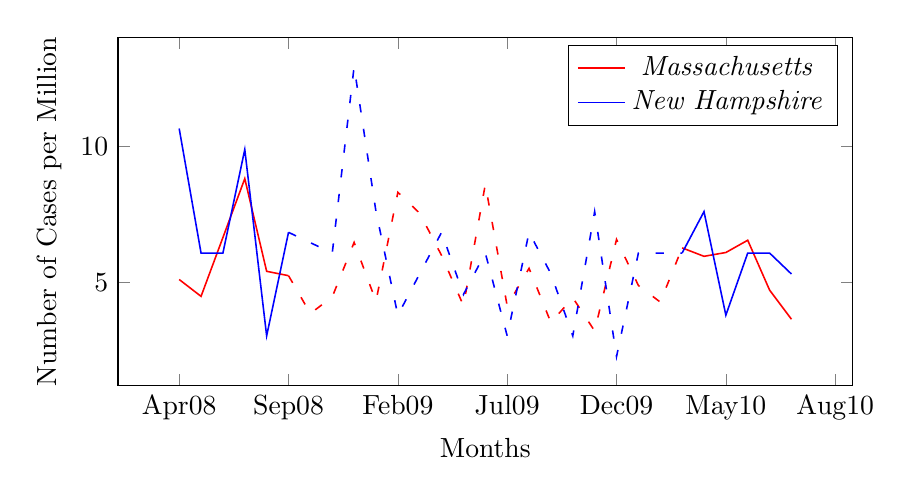
\begin{tikzpicture}
\begin{axis}[
  legend entries = {\textit{Massachusetts},,,,,\textit{New Hampshire}},
    xlabel={Months},
    ylabel={Number of Cases per Million},
    width=0.9\textwidth,
    height=6cm,
    symbolic x coords={Apr08,May08,Jun08,Jul08,Aug08,Sep08,Oct08,Nov08,Dec08,Jan09,Feb09,Mar09,Apr09,May09,Jun09,Jul09,Aug09,Sep09,Oct09,Nov09,Dec09,Jan10,Feb10,
    Mar10,Apr10,May10,Jun10,Jul10,Aug10}
]


\addplot[line width=0.20mm, color=red]
    coordinates{(Apr08, 5.11) (May08, 4.49) (Jun08, 6.65) (Jul08, 8.81) (Aug08, 5.41) (Sep08, 5.25)
    };

\addplot[line width=0.20mm, color=red,loosely dashed]
    coordinates{(Sep08, 5.25) (Oct08, 3.86) (Nov08, 4.47) (Dec08, 6.47) (Jan09, 4.31) (Feb09, 8.31) (Mar09, 7.54) (Apr09, 5.99) (May09, 4.15) (Jun09, 8.60) (Jul09, 4.14) (Aug09, 5.52) (Sep09, 3.53) (Oct09, 4.44) (Nov09, 3.22) (Dec09, 6.58) (Jan10, 4.89) (Feb10, 4.28) (Mar10, 6.27)
    };

\addplot[line width=0.20mm, color=red]
    coordinates{(Mar10, 6.27) (Apr10, 5.96) (May10, 6.10) (Jun10, 6.55) (Jul10, 4.72) (Aug10, 3.65)
    };

\addplot[line width=0.20mm, color=blue]
    coordinates{(Apr08, 10.65) (May08, 6.08) (Jun08, 6.08) (Jul08, 9.88) (Aug08, 3.04) (Sep08, 6.84)
    };

\addplot[line width=0.20mm, color=blue,loosely dashed]
    coordinates{(Sep08, 6.84) (Nov08,  6.08) (Dec08, 12.92) (Jan09, 7.60) (Feb09, 3.80) (Mar09, 5.32) (Apr09, 6.84) (May09, 4.56) (Jun09, 6.08) (Jul09, 3.04) (Aug09, 6.84) (Sep09, 5.32) (Oct09, 3.04) (Nov09, 7.60) (Dec09, 2.28) (Jan10, 6.08) (Feb10, 6.08) (Mar10, 6.08)
    };

\addplot[line width=0.20mm, color=blue]
    coordinates{(Mar10, 6.08) (Apr10, 7.60) (May10, 3.80) (Jun10, 6.08) (Jul10, 6.08) (Aug10, 5.31)
    };

\end{axis}
\end{tikzpicture}
\end{figure}
\end{frame}


\begin{frame}{Massachusetts Data Security Law (2 of 2)}
\begin{figure}
      \caption{Comparing Massachusetts and North Carolina (1000+ residents)} \label{fig:figure12}
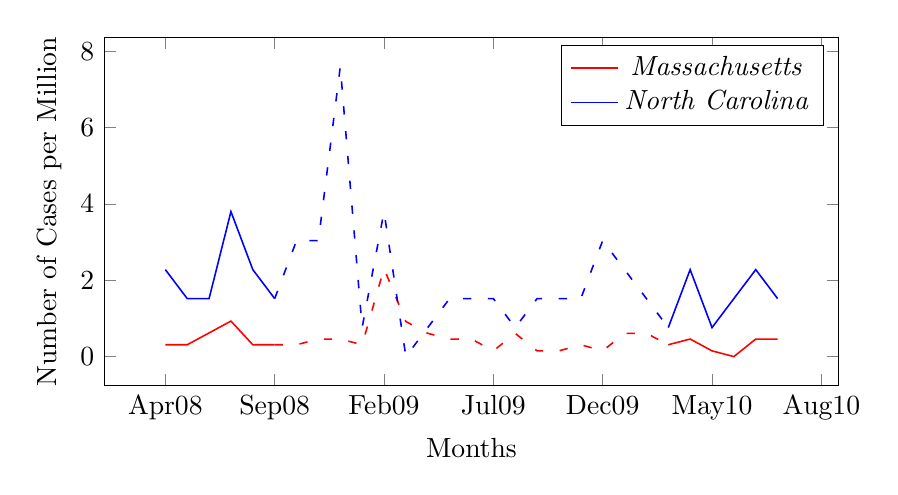
\begin{tikzpicture}
\begin{axis}[
  legend entries = {\textit{Massachusetts},,,,,\textit{North Carolina}},
    xlabel={Months},
    ylabel={Number of Cases per Million},
    width=0.9\textwidth,
    height=6cm,
    symbolic x coords={Apr08,May08,Jun08,Jul08,Aug08,Sep08,Oct08,Nov08,Dec08,Jan09,Feb09,Mar09,Apr09,May09,Jun09,Jul09,Aug09,Sep09,Oct09,Nov09,Dec09,Jan10,Feb10,
    Mar10,Apr10,May10,Jun10,Jul10,Aug10}
]
 
\addplot[line width=0.20mm, color=red]
    coordinates{(Apr08, 0.31) (May08, 0.31) (Jun08, 0.62) (Jul08, 0.93) (Aug08, 0.31) (Sep08, 0.31)
    };

\addplot[line width=0.20mm, color=red,loosely dashed]
    coordinates{(Sep08, 0.31) (Oct08, 0.31) (Nov08, 0.46) (Dec08, 0.46) (Jan09, 0.31) (Feb09, 2.31) (Mar09, 0.92) (Apr09, 0.61) (May09, 0.46) (Jun09, 0.46) (Jul09, 0.15) (Aug09, 0.61) (Sep09, 0.15) (Oct09, 0.15) (Nov09, 0.31) (Dec09, 0.15) (Jan10, 0.61) (Feb10, 0.61) (Mar10, 0.31)
    };

\addplot[line width=0.20mm, color=red]
    coordinates{(Mar10, 0.31) (Apr10, 0.46) (May10, 0.15) (Jun10, 0) (Jul10, 0.46) (Aug10, 0.46)
    };

\addplot[line width=0.20mm, color=blue]
    coordinates{(Apr08, 2.28) (May08, 1.52) (Jun08, 1.52) (Jul08, 3.80) (Aug08, 2.28) (Sep08, 1.52)
    };

\addplot[line width=0.20mm, color=blue, loosely dashed]
    coordinates{(Sep08, 1.52) (Oct08, 3.04) (Nov08, 3.04) (Dec08, 7.60) (Jan09, 0.76) (Feb09, 3.80) (Mar09, 0) (Apr09, 0.76) (May09, 1.52) (Jun09, 1.52) (Jul09, 1.52) (Aug09, 0.76) (Sep09, 1.52) (Oct09, 1.52) (Nov09, 1.52) (Dec09, 3.04) (Jan10, 2.28) (Feb10, 1.52) (Mar10, 0.76)
    };

\addplot[line width=0.20mm, color=blue]
    coordinates{(Mar10, 0.76) (Apr10, 2.28) (May10, 0.76) (Jun10, 1.52) (Jul10, 2.28) (Aug10, 1.52)
    };


\end{axis}
\end{tikzpicture}
\end{figure}
\end{frame}


\begin{frame}{HITECH Act (1 of 2)}
\begin{figure}
      \caption{Comparing Health vs Non-Health Breaches} \label{fig:figure12}
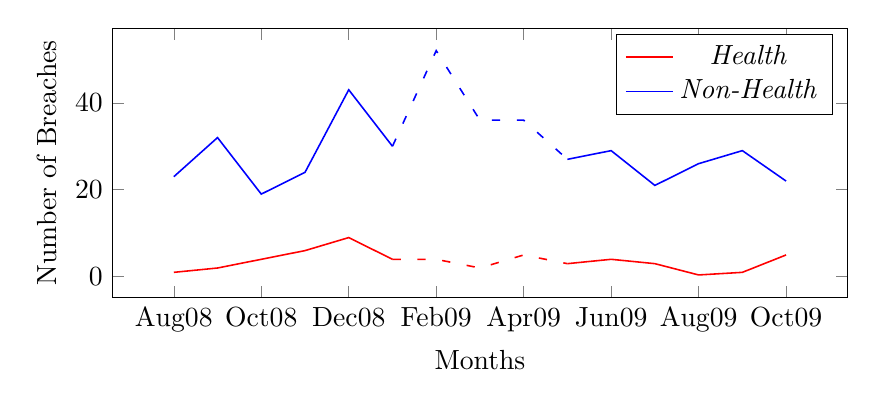
\begin{tikzpicture}
\begin{axis}[
  legend entries = {\textit{Health},,,,,\textit{Non-Health}},
    xlabel={Months},
    ylabel={Number of Breaches},
    width=0.9\textwidth,
    height=5cm,
    symbolic x coords={Aug08, Sep08, Oct08, Nov08, Dec08, Jan09, Feb09, Mar09, Apr09, May09, Jun09, Jul09, Aug09, Sep09, Oct09, Nov09},
]
 
\addplot[line width=0.20mm, color=red]
    coordinates{(Aug08, 1) (Sep08, 2) (Oct08, 4) (Nov08, 6) (Dec08, 9) (Jan09, 4)
    };

\addplot[line width=0.20mm, color=red,loosely dashed]
    coordinates{(Jan09, 4) (Feb09, 4) (Mar09, 2) (Apr09, 5) (May09, 3) 
    };

\addplot[line width=0.20mm, color=red]
    coordinates{(May09, 3) (Jun09, 4) (Jul09, 3) (Aug09, 0.4) (Sep09, 1) (Oct09, 5)
    };
    
\addplot[line width=0.20mm, color=blue]
    coordinates{(Aug08, 23) (Sep08, 32) (Oct08, 19) (Nov08, 24) (Dec08, 43) (Jan09, 30)
    };

\addplot[line width=0.20mm, color=blue,loosely dashed]
    coordinates{(Jan09, 30) (Feb09, 52) (Mar09, 36) (Apr09, 36) (May09, 27)
    };

\addplot[line width=0.20mm, color=blue]
    coordinates{(May09, 27) (Jun09, 29) (Jul09, 21) (Aug09, 26) (Sep09, 29) (Oct09, 22)
    };

\end{axis}
\end{tikzpicture}
\end{figure}
\end{frame}


\begin{frame}{HITECH Act (2 of 2)}
\begin{figure}
      \caption{Comparing Health vs Finance Breaches} \label{fig:figure12}
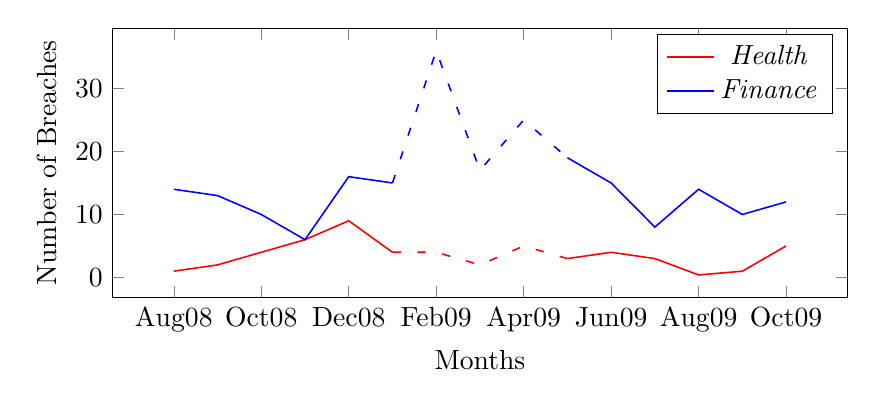
\begin{tikzpicture}
\begin{axis}[
  legend entries = {\textit{Health},,,,,\textit{Finance}},
    xlabel={Months},
    ylabel={Number of Breaches},
    width=0.9\textwidth,
    height=5cm,
    symbolic x coords={Aug08,Sep08,Oct08,Nov08,Dec08,Jan09,Feb09,Mar09,Apr09,May09,Jun09,Jul09,Aug09,Sep09,Oct09,Nov09}
]
 
\addplot[line width=0.20mm, color=red]
    coordinates{(Aug08, 1) (Sep08, 2) (Oct08, 4) (Nov08, 6) (Dec08, 9) (Jan09, 4)
    };

\addplot[line width=0.20mm, color=red,loosely dashed]
    coordinates{(Jan09, 4) (Feb09, 4) (Mar09, 2) (Apr09, 5) (May09, 3)
    };

\addplot[line width=0.20mm, color=red]
    coordinates{(May09, 3) (Jun09, 4) (Jul09, 3) (Aug09, 0.4) (Sep09, 1) (Oct09, 5)
    };
    
\addplot[line width=0.20mm, color=blue]
    coordinates{(Aug08, 14) (Sep08, 13) (Oct08, 10) (Nov08, 6) (Dec08, 16) (Jan09, 15)
    };

\addplot[line width=0.20mm, color=blue,loosely dashed]
    coordinates{(Jan09, 15) (Feb09, 36) (Mar09, 17) (Apr09, 25) (May09, 19)
    };

\addplot[line width=0.20mm, color=blue]
    coordinates{(May09, 19) (Jun09, 15) (Jul09, 8) (Aug09, 14) (Sep09, 10) (Oct09, 12)
    };

\end{axis}
\end{tikzpicture}
\end{figure}
\end{frame}

\begin{frame}{Wyndham FTC Suit Initial Complaint}
    \begin{figure}[!htb]
      \caption{The Wyndham FTC Suit as Intervention} \label{fig:FTCWyndham}
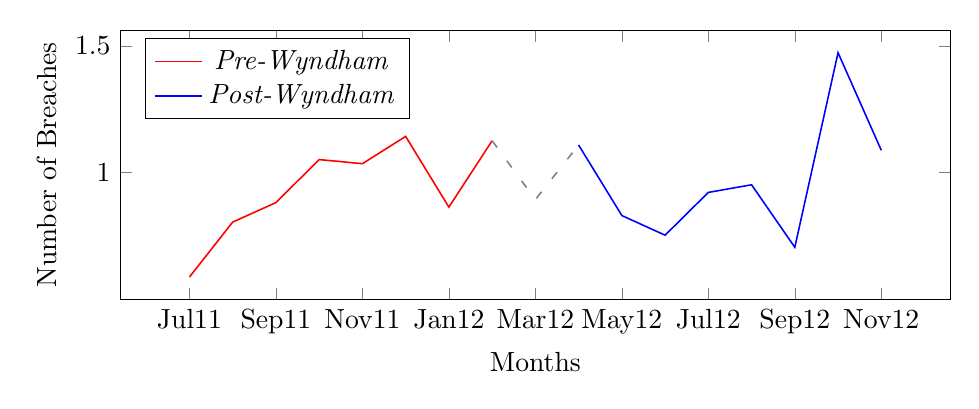
\begin{tikzpicture}
\begin{axis}[
  legend entries = {\textit{Pre-Wyndham},,\textit{Post-Wyndham}}, legend pos=north west,
    xlabel={Months},
    ylabel={Number of Breaches},
    width=\textwidth,
    height=5cm,
    symbolic x coords={Jul11,Aug11,Sep11,Oct11,Nov11,Dec11,Jan12,Feb12,Mar12,Apr12,May12,Jun12,Jul12,Aug12,Sep12,Oct12,Nov12}]

\addplot[line width=0.20mm, color=red]
    coordinates{(Jul11, 0.588938) (Aug11, 0.8053679) (Sep11, 0.8822077) (Oct11, 1.0517442) (Nov11, 1.0355747) (Dec11, 1.1429940) (Jan12, 0.8643827)
    (Feb12, 1.1260221)};

\addplot[line width=0.20mm, color=gray,loosely dashed]
    coordinates{(Feb12, 1.1260221) (Mar12, 0.8940427) (Apr12, 1.1090831) 
    };

\addplot[line width=0.20mm, color=blue]
    coordinates{(Apr12, 1.1090831) (May12, 0.8312409) (Jun12, 0.753756) (Jul12, 0.9223338) (Aug12, 0.9524249) (Sep12, 0.7061537) (Oct12, 1.4727033) (Nov12,1.0884417)
    };

\end{axis}
\end{tikzpicture}
\end{figure}
\end{frame}

\begin{frame}{Wyndham FTC Suit Third Circuit}
\begin{figure}[!htb]
    \caption{The Wyndham FTC Suit as Intervention (Third Circuit Decision)}
    \label{fig:FTCWyndham2}
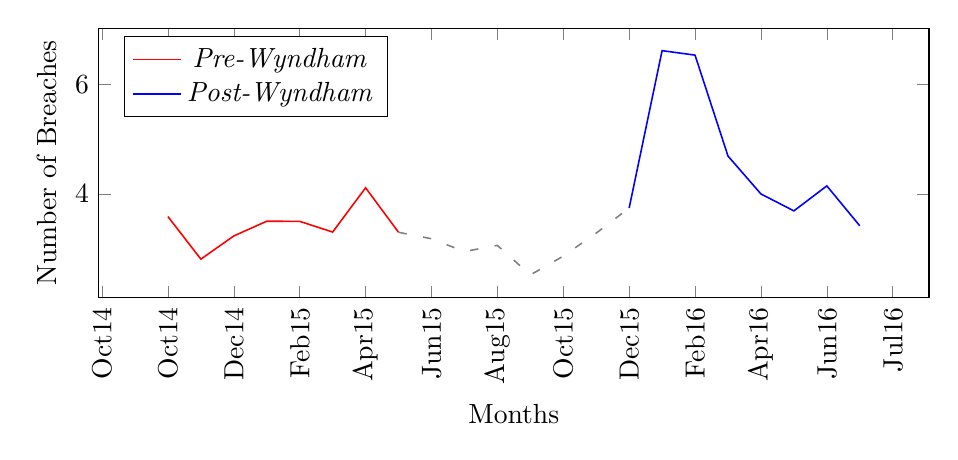
\begin{tikzpicture}
\begin{axis}[
  legend entries = {\textit{Pre-Wyndham},,\textit{Post-Wyndham}}, legend pos=north west,
    xlabel={Months},
    ylabel={Number of Breaches},
    width=\textwidth,
    height=5cm,
    symbolic x coords={Oct14,Nov14,Dec14,Jan15,Feb15,Mar15,Apr15,May15,Jun15,Jul15,Aug15,Sep15,Oct15,Nov15,Dec15,Jan16,Feb16,Mar16,Apr16,May16,Jun16,Jul16},
    x tick label style={rotate=90}]

\addplot[line width=0.20mm, color=red]
    coordinates{(Oct14, 3.582033) (Nov14, 2.801449) (Dec14, 3.227282) (Jan15, 3.497117)
    (Feb15, 3.494775) (Mar15, 3.298412) (Apr15,4.110562) (May15,3.294002)};

\addplot[line width=0.20mm, color=gray,loosely dashed]
    coordinates{(May15,3.294002) (Jun15, 3.175353) (Jul15, 2.940798) (Aug15, 3.054587) (Sep15, 2.511382) (Oct15, 2.856968) (Nov15,3.279193) (Dec15, 3.739336)
    };

\addplot[line width=0.20mm, color=blue]
    coordinates{ (Dec15, 3.739336) (Jan16, 6.625614) (Feb16, 6.543677) (Mar16, 4.692542) (Apr16,3.997214) (May16,3.686983) (Jun16, 4.144944) (Jul16, 3.413344)
    };
\end{axis}
\end{tikzpicture}
\end{figure}
\end{frame}

\begin{frame}{Quasi-Experiment for Wyndham FTC Suit, Third Circuit Decision}
\begin{table}[!htb]
    \caption{Quasi-Experiment for Wyndham FTC Suit, Third Circuit Decision}
    \label{tab:FTC_Wyndham2}
    \begin{tabular}{l|c|c|c|l}
      \textbf{Parameter} & \textbf{Interpretation} & \textbf{Estimate} & \textbf{Std Error} & \textbf{Probability}\\ % <-- added & and content for each column
      \hline
      $\alpha$ & Intercept & 3.16 &  0.67 &  0.00 *** \\  \hline % <--
      $\beta_1$ & Pre-Trend & 0.06 & 0.13 & 0.68  \\  \hline % <--
      $\beta_2$ & Post-Level & 2.28 & 0.87 & 0.02 * \\ % <--
      & Change & & & \\ \hline
      $\beta_3$ & Post-Trend & -0.34 & 0.19 & 0.09 $\cdot$ \\ % <--
      & Change & & & \\
    \end{tabular}
\end{table}
\end{frame}

\section{Implications}

\begin{frame}{Estimate of Saving from NY DFS Regulations}
    \begin{figure}
      \caption{Savings from Regulation over 1 Year} \label{fig:savings_est}
    \centering
    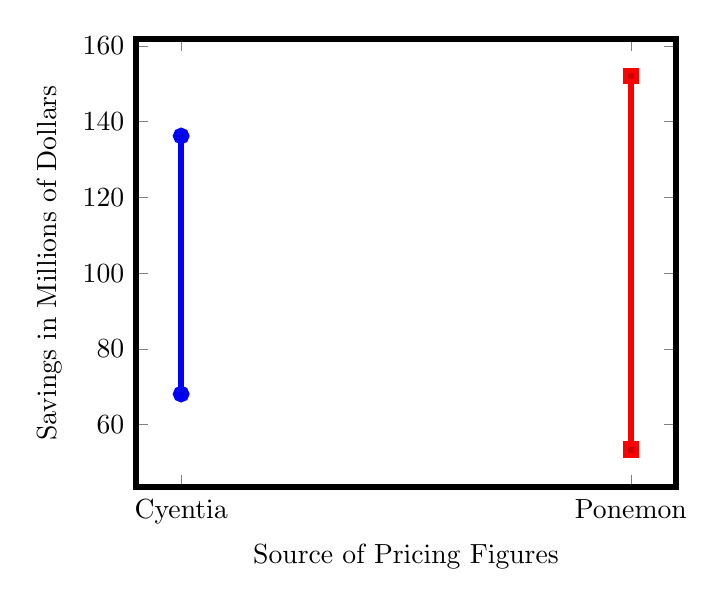
\begin{tikzpicture}
      \begin{axis}[
        line width=0.07cm,
        % enlarge y limits={abs=0.45cm},
        xlabel={Source of Pricing Figures},
        ylabel={Savings in Millions of Dollars},
        symbolic x coords={Cyentia, Ponemon},
        xtick={Cyentia, Ponemon},
]
      \addplot coordinates {(Cyentia, 68.10) (Cyentia, 136.2)};
      \addplot coordinates {(Ponemon, 53.39) (Ponemon, 151.99) };
      \end{axis}
\end{tikzpicture}
\end{figure}
\end{frame}

\begin{frame}{Question of Persistence of Breach Reduction}
\begin{figure}[!htb]
      \caption{New York Financial Breach Growth in 2020} \label{fig:NY_Continued}
      \resizebox{\textwidth}{!}{
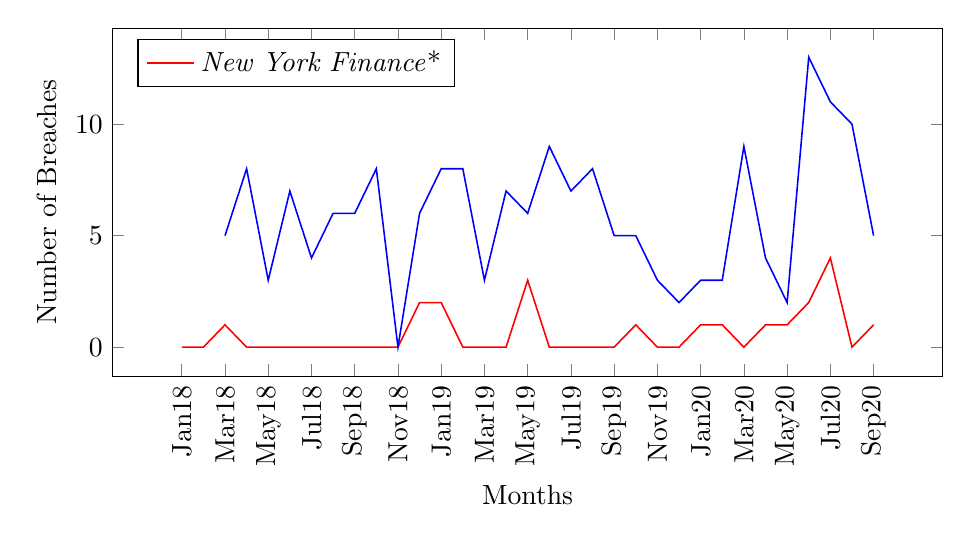
\begin{tikzpicture}
\begin{axis}[
  legend entries = {\textit{New York Finance}*,,,,,\textit{Not-New York Finance}**}, legend pos=north west,
    xlabel={Months},
    ylabel={Number of Breaches},
    width=\textwidth,
    height=6cm,
    symbolic x coords={Jan18,Feb18,Mar18,Apr18,May18,Jun18,Jul18,Aug18,Sep18,Oct18,Nov18,Dec18,Jan19,Feb19,Mar19,Apr19,May19,Jun19,Jul19,Aug19,Sep19,Oct19,Nov19,Dec19,Jan20,Feb20,Mar20,Apr20,May20,Jun20,Jul20,Aug20,Sep20},
    xtick={Jan18,Mar18,May18,Jul18,Sep18,Nov18,Jan19,Mar19,May19,Jul19,Sep19,Nov19,Jan20,Mar20,May20,Jul20,Sep20},
    x tick label style={rotate=90}
    ].

\addplot[line width=0.20mm,color=red]
    coordinates{
    (Jan18, 0) (Feb18,0) (Mar18,1) (Apr18,0) (May18,0) (Jun18,0) (Jul18,0) (Aug18,0) (Sep18,0) (Oct18,0) (Nov18,0) (Dec18,2) (Jan19,2) (Feb19,0) (Mar19,0) (Apr19,0) (May19,3) (Jun19,0) (Jul19,0) (Aug19,0) (Sep19,0) (Oct19,1) (Nov19,0) (Dec19,0) (Jan20,1) (Feb20,1) (Mar20,0) (Apr20,1) (May20,1) (Jun20,2) (Jul20,4) (Aug20,0) (Sep20,1)
    };

\addplot[line width=0.20mm,color=blue]
    coordinates{(Mar18,5) (Apr18,8) (May18,3) (Jun18,7) (Jul18,4) (Aug18,6) (Sep18,6) (Oct18,8) (Nov18,0) (Dec18,6) (Jan19,8) (Feb19,8) (Mar19,3) (Apr19,7) (May19,6) (Jun19,9) (Jul19,7) (Aug19,8) (Sep19,5) (Oct19,5) (Nov19,3) (Dec19,2) (Jan20,3) (Feb20,3) (Mar20,9) (Apr20,4) (May20,2) (Jun20,13) (Jul20,11) (Aug20,10) (Sep20,5)
    };
    
\end{axis}
\end{tikzpicture}}
\end{figure}
\end{frame}


\begin{frame}{Regulatory Requirements}
\begin{table}[!htb]
  \caption{Organizational Regulatory Requirements}
  \resizebox{\textwidth}{!}{
  \label{tab:org_reg}
\begin{tabular}{|l|l|l|l|l|}
\hline
& \begin{tabular}[c]{@{}l@{}}MA Data\\ Security Law\end{tabular} & HITECH Act & \begin{tabular}[c]{@{}l@{}}FTC Section 5\\ (Wyndham Hotel)\end{tabular} & \begin{tabular}[c]{@{}l@{}}NY Dept of\\ Financial Services\end{tabular} \\ \hline
Designation of specific personnel         & Yes     & No     & No     & Yes \\ \hline
Education and training of employees       & Yes     & No     & No     & Yes \\ \hline
\begin{tabular}[c]{@{}l@{}}Creation and maintenance of\\ cyber policies\end{tabular}     & Yes     & No     & No     & Yes  \\ \hline
Notification of Breaches     & Yes/No\footnote{The initial law included a notification requirement, however the cybersecurity provisions were implemented later.}      & Yes     & No     & Yes \\ \hline
Certification of compliance      & No      & No     & No     & Yes \\ \hline
\end{tabular}}
\end{table}
\end{frame}

\begin{frame}{Computer Security Requirements}
\begin{table}[!htb]
  \caption{Computer Security Requirements}
  \resizebox{\textwidth}{!}{
  \label{tab:comp_sec}
\begin{tabular}{|l|l|l|l|l|}
\hline
& \begin{tabular}[c]{@{}l@{}}MA Data\\ Security Law\end{tabular} & HITECH Act & \begin{tabular}[c]{@{}l@{}}FTC Section 5\\ (Wyndham Hotel)\end{tabular} & \begin{tabular}[c]{@{}l@{}}NY Dept of\\ Financial Services\end{tabular} \\ \hline
Secure user authentication protocols      & Yes     & No     & Yes/No\footnotemark[5]     & Yes     \\ \hline
Secure access control measures       & Yes     & No     & Yes/No\footnotemark[5]     & Yes     \\ \hline
Encryption requirements        & Yes     & Yes        & Yes     & Yes  \\ \hline
\begin{tabular}[c]{@{}l@{}}Reasonably up-to-date security \\ software, patches, virus definitions\end{tabular} & Yes     & No     & Yes/No\footnote{Cited in the FTC's complaint against Wyndham, but also employed in prior actions}     & Yes     \\ \hline
Control third-party access to network     & Yes     & No     & Yes     & Yes \\ \hline
\multicolumn{5}{c}{} \\
\end{tabular}}
\end{table}
\end{frame}

\begin{frame}{Summary}
\begin{columns}
    \column{0.5\textwidth}
    \begin{itemize}
    \item The NY DFS cyber regulations had the strictest organizational and technical requirements.
    \item The NY DFS cyber regulations while effective, may not be persistent.
    \item Overall, there is mixed to limited evidence for the efficacy of US regulatory cyber policy  interventions.
    \item Tools of policy evaluation, like quasi-experiments, can be applied to cybersecurity policy interventions.
    \end{itemize}
    
    \column{0.5\textwidth}
    \begin{figure}
	\includegraphics[width=\textwidth]{Figures/us-capitol.jpg}
    \end{figure}  
\end{columns}
\end{frame}

{\setbeamercolor{palette primary}{fg=black, bg=white}
\begin{frame}[standout]
  Questions?
\end{frame}
}

%\appendix

\begin{frame}{Massachusetts Data Security Law}
  \begin{columns}
    \column{0.5\textwidth}
      \metroset{block=fill}
      \begin{exampleblock}{MA Data Security Law}
        Official Title: (201 CMR 17) Standards for the protection of personal information of residents of the Commonwealth
        \begin{center}Policy Impact\end{center}
        \begin{itemize}
            \item{Applies to anyone with  personal  information about  a  resident  of  the  Commonwealth}
            \item{Mandates companies develop, implement, and maintain a comprehensive information security program} 
        \end{itemize}
      \end{exampleblock}
      
    \column{0.5\textwidth}
    \textbf{Regulator:} Massachusetts Office of Consumer Affairs and Business Regulation
    \begin{figure}
	\includegraphics[width=\textwidth]{Figures/OCABR.jpg}
    \end{figure}
    \end{columns}
\end{frame}

\begin{frame}{HITECH Act}
    \begin{columns}
        \column{0.5\textwidth}
          \metroset{block=fill}
          \begin{exampleblock}{HITECH Act}
            Official Title: Health Information Technology for Economic and Clinical Health Act \\
            Part of the American Recovery and Reinvestment Act of 2009
            \begin{center}Policy Impact\end{center}
            \begin{itemize}
            \item{Amended the HIPAA Security Rule on personal health data}
            \item{Mandates Breach Notification when 500+ individuals affected}
            \end{itemize}
          \end{exampleblock}
          
        \column{0.5\textwidth}
        \textbf{Regulator:} United States Department of Health and Human Services
        \begin{figure}
    	\includegraphics[width=\textwidth]{Figures/hhs_logo_large.png}
        \end{figure}
    \end{columns}
\end{frame}


\begin{frame}{NY DFS Regulations}
  \begin{columns}
    \column{0.5\textwidth}
      \metroset{block=fill}
      \begin{exampleblock}{NY DFS Regulations}
        Official Title: 23 NYCRR 500 - Cybersecurity Requirements for Financial Services Companies
        \begin{center}Policy Impact\end{center}
        \begin{itemize}
        \item{Requires certification of compliance with NY State}
        \item{Mandates policies, procedures, and risk assessments}
        \end{itemize}
      \end{exampleblock}
    \column{0.5\textwidth}
    \textbf{Regulator:} New York Department of Financial Services
        \begin{figure}
    	\includegraphics[width=\textwidth]{Figures/NY_DFS.jpg}
        \end{figure}    
  \end{columns}
\end{frame}

\begin{frame}{FTC Section 5}
  \begin{columns}
    \column{0.5\textwidth}

      \metroset{block=fill}
      \begin{exampleblock}{FTC Section 5}
        Official Title: Section 5(a) of the Federal Trade Commission Act (15 USC §45)
        \begin{center}Policy Impact\end{center}
        \begin{itemize}
        \item{Prohibits “unfair or deceptive  acts  or  practices  in  or  affecting commerce.”}
        \item{Data security orders require a comprehensive information security program}
        \end{itemize}
      \end{exampleblock}
    \column{0.5\textwidth}
    \textbf{Regulator:} United States Federal Trade Commission 
    \begin{figure}
	\includegraphics[width=\textwidth]{Figures/FTC.jpg}
    \end{figure}    
    \end{columns}
\end{frame}

\begin{frame}{FTC Section 5}
\begin{figure}
      \caption{FTC Data Breach Enforcement Cases per Year} \label{fig:figure12}
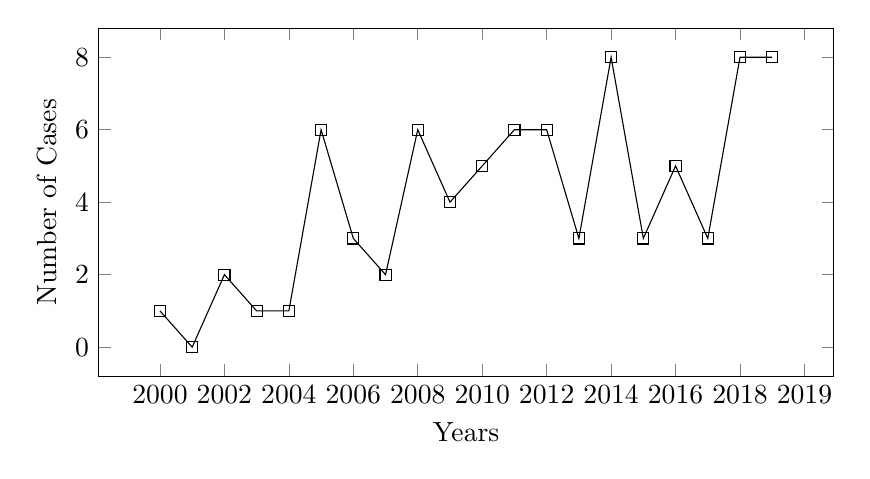
\begin{tikzpicture}
\begin{axis}[
    xlabel={Years},
    ylabel={Number of Cases},
    width=0.9\textwidth,
    height=6cm,
    symbolic x coords={2000,2001,2002,2003,2004,2005,2006,2007,2008,2009,2010,2011,2012,2013,2014,2015,2016,2017,2018,2019}
]
 
\addplot[
    mark=square,
    ]
    coordinates{(2000,1) (2001,0) (2002,2) (2003,1) (2004,1) (2005,6) (2006,3) (2007,2) (2008,6) (2009,4) (2010,5) (2011,6) (2012,6) (2013,3) (2014,8) (2015,3) (2016,5)	(2017,3)	(2018,8)	(2019,8)
    };
 
\end{axis}
\end{tikzpicture}
\end{figure}
\textbf{Source:} FTC Cases and Proceedings Advanced Search, Tagged as Data Security Topic
\end{frame}

\begin{frame}{Command and Control vs Meta-Regulations}
\begin{quote}
`\textbf{Command and control}' regulation, which refers to the prescriptive nature of the regulation (the command) supported by the imposition of some negative action by the regulator (the control) ... If adequately enforced, command and control regulation is dependable; it can specify operational parameters and regulatory obligations with clarity and immediacy.
\end{quote}
\vspace{.15cm}
\begin{quote}
`\textbf{Meta-regulation}' has been used to describe regulation for self-regulation in different ways. At its most basic, it relates to corporate self-audits and safety cases where businesses develop their own rules and reporting for the regulator to assess.    
\end{quote}
%\begin{flushright}
 -F.C. Simon, 2017 \cite{SimonMetaregulationpracticenormative2016}
%\end{flushright}
\end{frame}

\begin{frame}{Background: Breach Notification Laws}
  \begin{figure}
      \caption{States and Territories with Breach Notification Laws in Place by Year}
    \begin{tikzpicture}
      \begin{axis}[
        mbarplot,
        xlabel={Years},
        ylabel={States with Law},
        width=0.9\textwidth,
        height=6cm,
        symbolic x coords={2002,2003,2004,2005,2006,2007,2008,2009,2010,2011,2012,2013,2014,2015,2016,2017,2018,2019}
      ]
      \addplot plot coordinates {(2002,1) (2003,1) (2004,1) (2005,18) (2006,34) (2007,39) (2008,45) (2009,46) (2010,47) (2011,47) (2012,47) (2013,47) (2014,49) (2015,49) (2016,49)	(2017,50)	(2018,52)	(2019,52)};
      \end{axis}
    \end{tikzpicture}
  \end{figure}
\textbf{Source:} \href{https://www.itgovernanceusa.com/data-breach-notification-laws}{IT Governance USA Inc}
\end{frame}


\begin{frame}{Literature Review: Datasets (Continued)}
  \begin{figure}
      \caption{Data Breach Incidents by Year in Public Datasets} \label{fig:figure5}
    \begin{tikzpicture}
      \begin{axis}[
        mbarplot,
        xlabel={Years},
        ylabel={Breach Incidents},
        legend style={at={(0.5,-0.3)},anchor=north,legend columns=-1},
        width=0.9\textwidth,
        height=6cm,
        symbolic x coords={2005,2006,2007,2008,2009,2010,2011,2012,2013,2014,2015,2016,2017,2018, 2019}
      ]
      \addplot plot coordinates {(2005,88) (2006,407) (2007,383) (2008,298) (2009,219) (2010,700) (2011,631) (2012,650) (2013,674) (2014,548) (2015,355) (2016,419)	(2017,303)	(2018,765) (2019, 40)};
      \addplot plot coordinates {(2005,) (2006,) (2007,) (2008,) (2009,18) (2010,191) (2011,182) (2012,201) (2013,248) (2014,275) (2015,213) (2016,214)	(2017,210)	(2018,206) (2019, 198)};      
      \legend{Clearinghouse, HHS}
      \end{axis}
    \end{tikzpicture}
  \end{figure}
\end{frame}

\begin{frame}{Variables}
\begin{itemize}
\item Dependent variables
    \begin{itemize}
    \item Reports of Data Breaches to the States
    \item Identity Theft Reports (FTC Consumer Sentinel Network)
    \item Cybersecurity Complaints (FBI Internet Crime Complaint Center)
    \end{itemize}
\item Independent variables
    \begin{itemize}
    \item Changes in Breach Reporting Requirements
    \item Cyber Hygiene (CyberGreen)
    \item Vulnerability (NVD Scores)
    \item Cybersecurity Spending (Taxpayers for Commons Sense, OMB)
    \end{itemize}
\end{itemize}
\end{frame}

\begin{frame}{Dependent Variable: Identity Theft}
    \begin{figure}
    \caption{Identity Theft Reports Per Capita in 2018 (FTC)}    \label{fig:map2}
    \resizebox{\textwidth}{!}{
    \begin{tikzpicture}
    \tikzset{set state val/.style args={####1/####2}{####1={fill=blue!####2}}}
    \tikzset{set state val/.list={AL/45.9, AK/29.6, AZ/50.3, AR/29.9, CA/75.9, CO/44.1, CT/44.2, DE/64.2, DC/69.5, FL/73.9, GA/100, HI/28.8, ID/30.4, IL/53.8, IN/30, IA/21.1, KS/30.4, KY/23.4, LA/49.2, ME/21.9, MD/60, MA/36.8, MI/54.5, MN/29.2, MS/41.9, MO/35.6, MT/29.6, NE/26.8, NV/78.4, NH/45.5, NJ/51.1, NM/40, NY/49.8, NC/45, ND/24.3, OH/35.3, OK/32.8, OR/39.8, PA/44.3, RI/38.4, SC/52.7, SD/21.3, TN/41.8, TX/66.8, UT/37.3, VT/20.1, VA/39.6, WA/40.2, WV/23.5, WI/25.6, WY/23.1}}
    \USA[every state={draw=white, ultra thick, fill=black!10}]
    \matrix [draw,below left] at (current bounding box.north west) {
    \node [fill=blue!80,label=right:Higher Per-Capita] {}; \\
    \node [fill=blue!40,label=right:Lower Per-Capita] {}; \\
    };
    \end{tikzpicture}}
    \end{figure}
\end{frame}


\begin{frame}{Dependent Variable: Cybersecurity Complaints}
    \begin{figure}
    \caption{Cybersecurity Complaints Per Capita in 2018 (FBI IC3)}
    \label{fig:map3}
    \resizebox{\textwidth}{!}{
    \begin{tikzpicture}
    \tikzset{set state val/.style args={####1/####2}{####1={fill=purple!####2}}}
    \tikzset{set state val/.list={AL/43.2,AK/100,AZ/51.5,AR/28.2,CA/57,CO/75.3,CT/40.4,DE/42.7,DC/89.3,FL/51.8,GA/39.8,HI/35.6,ID/39.7,IL/36.4,IN/32.1,IA/28.9,KS/33.1,KY/29,LA/34.2,ME/28.6,MD/66.8,MA/41.1,MI/34.7,MN/35.3,MS/29,MO/41.4,MT/34.1,NE/28.7,NV/79.3,NH/35.8,NJ/43.6,NM/46.7,NY/42.7,NC/33.3,ND/27.8,OH/30.7,OK/30.8,OR/49.5,PA/37.9,RI/44.7,SC/32.3,SD/24.2,TN/37.9,TX/41,UT/44.3,VT/38.6,VA/79.9,WA/65.8,WV/28.3,WI/52.4,WY/39.6}}
    \USA[every state={draw=white, ultra thick, fill=black!10}]
    \matrix [draw,below left] at (current bounding box.north west) {
    \node [fill=purple!80,label=right:Higher Per-Capita] {}; \\
    \node [fill=purple!40,label=right:Lower Per-Capita] {}; \\
    };
    \end{tikzpicture}}
    \end{figure}
\end{frame}

\begin{frame}{Independent Variable: Changes in Data Breach Laws}
  \begin{columns}
    \column{0.5\textwidth}
      \begin{figure}
      \caption{Proposed Breach Notification Legislation} \label{fig:figure9}
    \begin{tikzpicture}
      \begin{axis}[
        mbarplot,
        xlabel={Years},
        ylabel={Bills},
        width=0.9\textwidth,
        height=6cm,
        symbolic x coords={2010,2011,2012,2013,2014,2015,2016,2017,2018}
      ]
      \addplot plot coordinates {(2010,33) (2011,32) (2012,23) (2013,39) (2014,55) (2015,75) (2016,67)	(2017,77)	(2018,153)};
      
      \end{axis}
    \end{tikzpicture}
  \end{figure}
    \column{0.5\textwidth}
  \begin{figure}
      \caption{New and Amended Data Breach Notification Laws} \label{fig:figure10}
    \begin{tikzpicture}
      \begin{axis}[
        mbarplot,
        xlabel={Years},
        ylabel={Laws},
        width=0.9\textwidth,
        height=6cm,
        symbolic x coords={2010,2011,2012,2013,2014,2015,2016,2017,2018}
      ]
      \addplot plot coordinates {(2010,2) (2011,5) (2012,3) (2013,1) (2014,15) (2015,18) (2016,5)	(2017,12)	(2018,31)};
      
      \end{axis}
    \end{tikzpicture}
  \end{figure}
  \end{columns}
\end{frame}

\begin{frame}{Independent Variable: Cybersecurity Spending}
  \begin{figure}
      \caption{Cybersecurity Dollars Spent by CFO Agencies in Billions per FY} \label{fig:figure11}
    \begin{tikzpicture}
      \begin{axis}[
        mbarplot,
        xlabel={Years},
        ylabel={Dollars in Billions},
        width=0.9\textwidth,
        height=6cm,
        symbolic x coords={2007,2008,2009,2010,2011,2012,2013,2014,2015,2016,2017,2018,2019}
      ]

      \addplot plot coordinates {(2007,5.4) (2008,6.2) (2009,8.2) (2010,10.2) (2011,10.7) (2012,12.9) (2013,13.3) (2014,20.0) (2015,21.6) (2016,25.9)	(2017,12.3)	(2018,13.5)	(2019,14.0)};
      
      \end{axis}
    \end{tikzpicture}
  \end{figure}
\textbf{Source:} Taxpayers for Common Sense ’07-’16, Office of Management and Budget ’17-’19
\end{frame}

\begin{frame}{Decomposition of Trends}
    \begin{figure}
   \label{fig:decomposition}
   \caption{Sample Decomposition of Additive Time Series for Massachusetts*}
	\includegraphics[width=\textwidth]{Figures/TimeDecomposition.jpg}
    \end{figure}
* Data breaches per Million in Massachusetts
\end{frame}


\begin{frame}{Case Implementation Period}
\begin{columns}
    \column{0.5\textwidth}
    \begin{enumerate}
      \item MA Data Security Law
          \begin{itemize}
              \item Enacted: September 22, 2008
              \item Enforcement: March 1, 2010
          \end{itemize}
      \item HITECH Act
            \begin{itemize}
                \item Enacted: February 17, 2009
                \item Enforcement: May 27, 2009
            \end{itemize}
      \item NY DFS regulations
          \begin{itemize}
              \item Enacted: March 1, 2017
              \item Enforcement: September 3, 2018 (Third Phase)
          \end{itemize}
    \end{enumerate}
    \column{0.5\textwidth}

    \begin{figure}
      \caption{Implementation Days} \label{fig:figure13}
    \begin{tikzpicture}
      \begin{axis}[
        mbarplot,
    xlabel={Policy},
    ylabel={Number of Days},
    width=0.9\textwidth,
    height=6cm,
    symbolic x coords={Policy 1, Policy 2, Policy 3}
]
      \addplot plot coordinates {(Policy 1, 525) (Policy 2, 99) (Policy 3, 531)};
      
      \end{axis}
\end{tikzpicture}
\end{figure}
\end{columns}
\end{frame}


\begin{frame}{Comparison of Regulatory Penalties}
\begin{columns}
    \column{0.5\textwidth}
    \begin{enumerate}
      \item MA Data Security Law
            \begin{itemize}
                \item Penalties have a maximum limit per violation of \$5,000 \\
            \end{itemize}
      \item HITECH Act
            \begin{itemize}
                \item Penalties are limited per violation at \$100 to \$50,000 \\
            \end{itemize}
      \item NY DFS regulations
          \begin{itemize}
                \item Penalties have a maximum limit per day of
                \begin{itemize}
                    \item \$2,500 (any-violation) \\
                    \item \$15,000 (negligence)\\
                    \item \$75,000 (knowing) \\
                \end{itemize}
          \end{itemize}
      \item FTC Enforcements
          \begin{itemize}
                \item Penalties have a maximum limit per violation of
                \begin{itemize}
                    \item \$16,000 (pre-2016) \\
                    \item \$40,000 (post-2016) \\
                \end{itemize}
          \end{itemize}          
    \end{enumerate}
    \column{0.5\textwidth}
\begin{figure}
      \caption{Maximum Penalty} \label{fig:figure14}
    \begin{tikzpicture}
      \begin{axis}[
        xlabel={Policy},
        ylabel={Cost in \$10,000 Dollars},
        width=0.9\textwidth,
        height=7cm,
        symbolic x coords={P1, P2, P3, P4}
]
      \addplot coordinates {(P1, 5000)};
      \addplot coordinates {(P2, 100) (P2, 50000)};
      \addplot coordinates {(P3, 2500) (P3, 15000) (P3, 75000)};   
      \addplot coordinates {(P4, 16000) (P4, 40000)};   
      \end{axis}
\end{tikzpicture}
\end{figure}
\end{columns}
\end{frame}


\begin{frame}[fragile]{Backup slides}
    \begin{figure}
      \caption{Population of States Reporting Breach Notifications} \label{fig:figure17}
    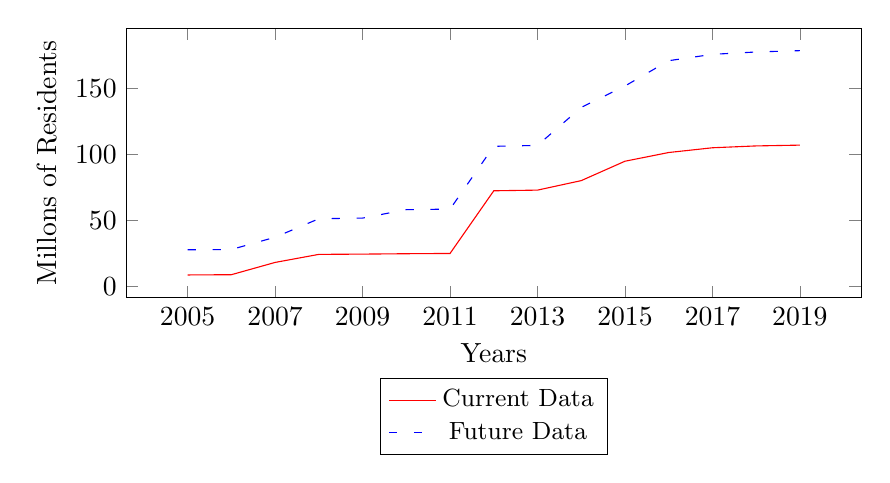
\begin{tikzpicture}
    \begin{axis}[legend style={font=\small, at={(0.5,-.3)},anchor=north},
    xlabel={Years},
    ylabel={Millons of Residents},
    width=0.9\textwidth,
    height=5cm,
    symbolic x coords={2005,2006,2007,2008,2009,2010,2011,2012,2013,2014,2015,2016,2017,2018,2019}
    ]
    \addplot[color=red]
    coordinates{(2005,8.7) (2006,8.9) (2007,18.2) (2008,24.3) (2009,24.5) (2010,24.8) (2011,25.0) (2012,72.5) (2013,73.0) (2014,80.2) (2015,94.9) (2016,101.5) (2017,105.1) (2018,106.5) (2019,107.1)};
    \addplot[color=blue,loosely dashed]
    coordinates{(2005,27.8) (2006,28.0) (2007,37.3) (2008,51.3) (2009,51.8) (2010,58.2) (2011,58.6) (2012,106.2) (2013,106.9) (2014,135.7) (2015,151.9) (2016,171.1) (2017,175.9) (2018,177.7) (2019,178.7)};
    \legend{Current Data, Future Data}
    \end{axis}
    \end{tikzpicture}
    \end{figure}
\end{frame}


\begin{frame}{Comparing New York Finance to New York Not-Finance with Maine Data}
    \begin{figure}[!htb]
    \caption{Comparing New York Finance to New York Not-Finance}
    \label{fig:ny_notfin}
    {
    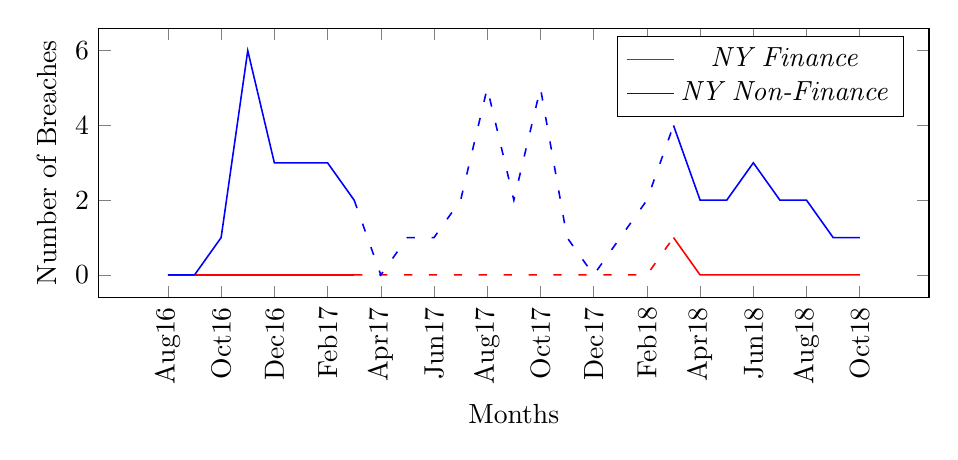
\begin{tikzpicture}
    \begin{axis}[
  legend entries = {\textit{NY Finance},,,,,\textit{NY Non-Finance}}, legend pos=north east,
    xlabel={Months},
    ylabel={Number of Breaches},
    width=\textwidth,
    height=5cm,
    symbolic x coords={Aug16,Sep16,Oct16,Nov16,Dec16,Jan17,Feb17,Mar17,Apr17,May17,Jun17,Jul17,Aug17,Sep17,Oct17,Nov17,Dec17,Jan18,Feb18,Mar18,Apr18,May18,Jun18,Jul18,Aug18,Sep18,Oct18},
    xtick={Aug16,Oct16,Dec16,Feb17,Apr17,Jun17,Aug17,Oct17,Dec17,Feb18,Apr18,Jun18,Aug18,Oct18},
    x tick label style={rotate=90}
    ].
\addplot[line width=0.20mm,color=red]
    coordinates{(Aug16,0) (Sep16,0) (Oct16,0) (Nov16,0) (Dec16,0) (Jan17,0) (Feb17,0) (Mar17,0)
    };
\addplot[line width=0.20mm,color=red,loosely dashed]
    coordinates{(Mar17,0) (Apr17,0) (May17,0) (Jun17,0) (Jul17,0) (Aug17,0) (Sep17,0) (Oct17,0) (Nov17,0) (Dec17,0) (Jan18,0) (Feb18,0) (Mar18,1)
    };
\addplot[line width=0.20mm,color=red]
    coordinates{(Mar18,1) (Apr18,0) (May18,0) (Jun18,0) (Jul18,0) (Aug18,0) (Sep18,0) (Oct18,0)
    };
\addplot[line width=0.20mm,color=blue]
    coordinates{(Aug16,0) (Sep16,0) (Oct16,1) (Nov16,6) (Dec16,3) (Jan17,3) (Feb17,3) (Mar17,2)
    };
\addplot[line width=0.20mm,color=blue,loosely dashed]
    coordinates{(Mar17,2) (Apr17,0) (May17,1) (Jun17,1) (Jul17,2) (Aug17,5) (Sep17,2) (Oct17,5) (Nov17,1) (Dec17,0) (Jan18,1) (Feb18,2) (Mar18,4)
    };
\addplot[line width=0.20mm,color=blue]
    coordinates{(Mar18,4) (Apr18,2) (May18,2) (Jun18,3) (Jul18,2) (Aug18,2) (Sep18,1) (Oct18,1)
    };
\end{axis}
\end{tikzpicture}}
\end{figure}
\end{frame}

\begin{frame}{Comparative ITS NY DFS Regulations (NY Finance Compared to NY Not-Finance with Maine Data}
\begin{table}[!htb]
  
    \label{tab:NY_NotFin_MA}
    \resizebox{\textwidth}{!}{
    \begin{tabular}{l|c|c|r|l}
      \textbf{Parameter} & \textbf{Interpretation} & \textbf{Estimate} & \textbf{Std Error} & \textbf{Probability}\\ % <-- added & and content for each column
      \hline
      $\alpha$ & Intercept & 0.54 & 0.79 & 0.50 \\  \hline % <--
      $\beta_1$ & Control Pre-Trend & 0.38 & 0.16 & 0.02 * \\  \hline % <--
      $\beta_2$ & Control Post-Level &  -0.01 & 1.02 & 0.99  \\ % <--
      & Change & & & \\ \hline
      $\beta_3$ & Control Post-Trend & -0.70 & 0.22 & 0.00 **\\ % <--
      & Change & & & \\ \hline
      $\beta_4$ & Treatment/Control & -0.54 & 1.11 & 0.63 \\ % <--
      & Pre-Level Difference & & & \\ \hline
      $\beta_5$ & Treatment/Control & -0.38 & 0.22 & 0.10 . \\ % <--
            & Pre-Trend Difference & & & \\ \hline
\rowcolor{yellow}      $\beta_6$ & Treatment/Control & 0.51 & 1.45 & 0.73 \\ % <--\
\rowcolor{yellow}            & Post-Level Difference & & & \\ \hline
\rowcolor{lightgray}      $\beta_7$ & Treatment/Control Change  & 0.62 & 0.31 & 0.06 . \\ % <--
\rowcolor{lightgray}            & in Slope Difference Pre-to Post- & & & \\ \hline
\end{tabular}}
\end{table}
\end{frame}


\begin{frame}[allowframebreaks]{References}

  \bibliography{references}
  \bibliographystyle{abbrv}

\end{frame}

\end{document}